\documentclass{article}
%\usepackage{arxiv}
\usepackage[numbers,sort&compress,super,comma]{natbib} % this must be before neurips_2024
\usepackage[]{neurips_2025}
\usepackage[utf8]{inputenc}
\usepackage[english]{babel}
\usepackage{amssymb, amsmath, amsthm, amsfonts}
\usepackage{thmtools, mathtools, mathrsfs, dsfont}
\usepackage{bbm}
%\usepackage{bbold} %for mathbb{1}
\usepackage{forloop}
\usepackage[pdftex]{graphicx}  %remove demo option in your document
\usepackage{sidecap}
\usepackage{enumerate}
\usepackage[shortlabels]{enumitem} %easy customization of itemize/enumerate lists
\PassOptionsToPackage{dvipsnames}{xcolor}
\usepackage{xcolor}
\definecolor{ForestGreen}{rgb}{0.13, 0.55, 0.13}
\definecolor{MidnightBlue}{rgb}{0.1, 0.1, 0.44}
\definecolor{BurntOrange}{rgb}{0.8, 0.33, 0.0}
\definecolor{Plum}{rgb}{0.56, 0.27, 0.52}
\usepackage[colorlinks=true,linkcolor=MidnightBlue,citecolor=ForestGreen,filecolor=TealBlue,urlcolor=Plum]{hyperref}
\hypersetup{breaklinks=true}
\usepackage{tikz}
\usetikzlibrary{positioning}
\usepackage{tikz-cd}


%for comments
\newcommand{\ptitle}[1]{\textbf{#1:}\xspace}
\definecolor{mpcolor}{rgb}{1, 0.1, 0.59}
\definecolor{ascolor}{rgb}{1, 0.5, 0.}
\newcommand{\mpcomment}[1]{\textcolor{mpcolor}{(#1)}}
\newcommand{\ascomment}[1]{\textcolor{ascolor}{(#1)}}

\graphicspath{{figures}}

\newtheorem{theorem}{Theorem}
\newtheorem{proposition}{Proposition}
\newtheorem{lemma}{Lemma}
\newtheorem{corollary}{Corollary}[theorem]
\theoremstyle{definition} \newtheorem{definition}{Definition}  \newtheorem{example}{Example}
\theoremstyle{remark} \newtheorem{remark}{Remark}


\newcommand{\reals}{\mathbb{R}}
\newcommand{\sep}{\operatorname{sep}}
\newcommand{\cl}{\operatorname{cl}}
\newcommand{\vol}{\operatorname{vol}}
\newcommand{\boa}{\operatorname{BoA}}
\newcommand{\mcN}{\mathcal{N}}
\newcommand{\mcK}{\mathcal{K}}
\newcommand{\mcU}{\mathcal{U}}
\newcommand{\mcX}{\mathcal{X}}
\newcommand{\T}{\operatorname{T}}
\newcommand{\TR}{\T\!\mathbb{R}}
\newcommand{\TM}{\T\!M}
\newcommand{\TpM}{\T_p\!M}
\newcommand{\Diff}{\operatorname{Diff}}
\newcommand{\Hpert}{H^{\text{pert}}}
\newcommand{\inv}{\operatorname{Inv}}
\newcommand{\manifold}{\mathcal{M}}

\newcommand{\defvec}[1]{\expandafter\newcommand\csname v#1\endcsname{{\mathbf{#1}}}}
\newcommand{\dm}[1]{\ensuremath{\mathrm{d}{#1}}} % dx dy dz dmu
\newcounter{ct}
\forLoop{1}{26}{ct}{
    \edef\letter{\alph{ct}}
    \expandafter\defvec\letter
}

% captial \vA
\forLoop{1}{26}{ct}{
    \edef\letter{\Alph{ct}}
    \expandafter\defvec\letter
}


%\title{Interpretable attractor motifs for a new language for neural computation}
%\title{Attractor motifs for an interpretable language for working memory-type neural computation}
%\title{Imposing interpretability of neural computation by extracting effective behavior through dynamical motifs}
%\title{Understanding working memory through canonical dynamical motifs}
\title{Canonical motif descriptions of memory maintenance neural computation}
%Dynamical Motif Extraction for Interpretable Neural Computation
% Interpretable Neural Computation via Dynamical Motifs
\author{\'Abel S\'agodi and Il Memming Park}
\date{\today}



\begin{document}
\maketitle

% keywords: interpretability, dynamical dissimilarity, dynamical motifs, neural computation, working memory, computation through dynamics

\begin{abstract}
The study of neural computation aims to understand the function of the brain as an information processing machine.
Neural systems are undoubtedly complex, necessitating principled and automated tools to abstract away details to organize and incrementally build intuition.
Systems with the same effective behavior can be abstracted by their representative member---one composed of asymptotic dynamical structures, while others are treated as imperfect realizations of this ideal canonical computation.
We propose a library of canonical computations and a new measure of dissimilarity that allows us to group systems based on their effective behavior by explicitly considering both deformations that break the topological conjugacy as well as diffeomorphisms that preserve it.
The proposed dissimilarity can be estimated from observed trajectories.
Numerical experiments demonstrate our methods ability to reconcile previously reported fragility of existing (dis)similarity measures for approximate continuous attractors and high-dimensional recurrent neural networks.
Although our experiments focus on working memory systems, the theoretical approach naturally extends to general mechanistic interpretation of recurrent dynamics in both biological and artificial neural systems.
We argue that abstract canonical computation motifs, rather than detailed dynamical systems, offer a more useful vocabulary for describing neural computation.
%
% Understanding neural computation in dynamical neural systems often requires interpreting the behavior of large, black-box models.
% This poses challenges for both interpretability and cross-model comparison—particularly when comparing models from different sources, such as two animals.
% To address this, we propose a framework for interpreting neural computation for working memory through \emph{dynamical motifs}—canonical, human-understandable building blocks of dynamics.
% Within this framework, we introduce a model reduction method that approximates the essential computational mechanism in a system by identifying small perturbations that render two systems topologically conjugate.
% Our method fits the homeomorphism that establishes the topological conjugacy as a Neural ODE.
% We derive measures of dissimilarity based on our homeomorphism-conjugacy mapping method.
% Our method uses a curated library of low-dimensional canonical motifs (e.g., limit cycles and various continuous attractors) to explain the core dynamics.
% This allows us to define and quantify similarity between systems in terms of shared dynamical structure.
% The extracted motifs are robust to parametric variation, suggesting they reflect stable computational strategies rather than model idiosyncrasies.
% We demonstrate the approach on various toy examples, most importantly approximate continuous attractors.
% Furthermore, we extract an approximate ring attractors from a high-dimensional RNNs trained on a angular velocity integration task, and show how the found homeomorphism captures the complexity of the geometry of the embedding of the ring.
% Our results highlight the utility of this method for robust interpretation and cross-system comparison within the computation-through-dynamics framework.
\end{abstract}

\section{Introduction}\label{sec:intro}
%Understanding the relationship between neural activity and behavior is a fundamental question in neuroscience.
Understanding neural computation requires more than capturing the details of neural dynamics; it necessitates the development of conceptual models that simplify and abstract the complexity of these processes into forms that are humanly interpretable.
Through abstraction and idealization, we can distill the essential features of neural activity, enabling meaningful understanding rather than merely presenting a detailed but opaque description.

%why no 20D attractors?
%Recent research has shown that, despite the inherent complexity of neuronal networks, their activity often resides on a low-dimensional manifold, representing only a small fraction of the system's full potential complexity \citep{duncker2021dynamics}.
%This empirical finding suggests that neural computation is governed by underlying constraints—potentially driven by task-relevant computations or external environmental factors—that allow for such a reduction in complexity.
%Such constraints not only make the idealization of neural systems feasible but also provide a path toward more interpretable models of neural activity.
 
%%%%
%\subsection{Memory maintenance in neural networks}\label{sec:ctd} 
Discovering how the brain contributes to behavior is the central aim of systems neuroscience.
We need a language that can describe how neural populations transform inputs into goal-directed behavior.
Here we focus on the memory maintenance part of this transformation.

Dynamical systems provide a powerful and widely used framework for studying neural computation, offering insights into cognitive functions such as working memory, short-term memory, and motor control \citep{beer1995ctrnn, beer2006parameterspace, sussillo2014neural, vyas2020ctd}.
In neural activity and in Recurrent Neural Networks (RNNs), computations are described by the dynamical properties of the network which are typically characterized by the dynamics asymptotic behavior or invariant sets.
Discrete and continuous forms of working memory, for example, can be modeled as attractor dynamics that stabilize persistent representations \citep{zhang2022translation, hoeller2024bridging}.
Short-term memory, involving transient yet structured activity, has been explored in dynamical models capturing task-dependent variability \citep{kurtkaya2025dynamical}.
% Motor control, too, exhibits low-dimensional dynamics shaped by recurrent structure \citep{wang2022representation}.
 While canonical models aim to distill these computations into minimal motifs \citep{chirimuuta2014minimal}, actual biological neural implementations may vary significantly, motivating the need for flexible yet interpretable abstractions.

Asymptotic behavior such as fixed points, limit cycles, and slow invariant manifolds are central to understanding how neural systems maintain memory over time.
Fixed-point attractors have long been used to characterize stable memory states in RNNs \citep{sussillo2013blackbox, katz2017fibers, golub2018fixedpointfinder}, while recent work highlights the role of limit cycles \citep{townley2000existence, pals2024inferring} and slow invariant manifolds in sustaining analog memory representations\citep{Sagodi2024a}.

%3 angles: neural activity, latent variable models, RNNs: all too obscure!!
Latent variable models have proven essential for extracting interpretable state space representations from high-dimensional neural activity \citep{zoltowski2020general, Dowling2024b, pei2neural}, enabling rigorous comparisons across systems \citep{libedinsky2023comparing} and supporting benchmarking efforts such as the Neural Latents and Computation-through-Dynamics (CtD) benchmarks \citep{pei2neural, versteeg2025computation}.
Within the computation-through-dynamics (CtD) framework, recurrent neural networks (RNNs) have emerged as powerful models for capturing both task-related computations \citep{yang2019task, yang2019multiple, yang2020artificial, sani2021nonlinearity} and the dynamical structure of cortical responses \citep{chaisangmongkon2017transience, mante2013context}.
These models support both top-down engineering approaches—where desired dynamics are imposed by construction \citep{eliasmith2003neuralengineering, eliasmith2005unified, eliasmith2010describe, pollock2020engineering, beiran2023rnns}—and bottom-up analysis of black-box systems trained for behavior \citep{sussillo2013blackbox, maheswaranathan2019reverse, golub2018fixedpointfinder, smith2021reverse, maheswaranathan2019universality, jarne2023initialization, nayebi2021heterogeneity, turner2021charting, turner2023simplicity, zhong2023mechanistic, huang2024measuring}.

Asymptotic behavior—captured by structures like fixed points, limit cycles, and slow manifolds—is central to memory maintenance in neural computation, encoding stable representations over time. However, in both latent variable models and task-trained RNNs, these structures are often embedded in high-dimensional, black-box dynamics, making them difficult to interpret \citep{whiteway2019interpretable,kar2022interpretability}. %obscurity
Identifying asymptotic structure is thus key to extracting interpretable, computationally meaningful mechanisms from complex neural models.
%lets bring some light!
Through abstraction and idealization, we can distill the essential features of neural activity, enabling understanding rather than merely presenting a detailed but opaque description.
This process is especially important in models where high-dimensional dynamics obscure the underlying computational structure, making interpretability contingent on identifying simplified, canonical representations. 

%The space of models for neural computation / the space of theories for neural computation
In this view, the space of theories for neural computation corresponds to the space of possible dynamical systems the brain might instantiate—a vast landscape.
Our method provides a means to chart regions of this space relevant for memory maintenance by identifying and parametrizing recurrent computations in a human-interpretable way.
This enables us to isolate families of dynamical motifs that serve as building blocks for memory-related neural dynamics, opening the door to theory-guided interpretability in complex models.
 
Here, we develop a data-driven method called Canonical Motif-based Dynamical Analysis (CMDA). 
In brief, CMDA returns a dissimilarity metric describing how a system compares to a dynamical motif both at the level of the topology of the dynamics and how much the dynamics needs to be transformed.
Our results demonstrate that CMDA identifies both dynamic structure and the complexity needed to deform it based on an interpretable motif.
This framework applies to core neural computations such as classification, working memory, and persistent representations (e.g., head direction cells).
It accommodates both infinite-horizon systems and finite-horizon systems like echo state networks, highlighting that time-limited trajectories may obscure deeper structural distinctions only visible in the full vector field.


%another perspective 
%Behavior, in many cases, is surprisingly simple. Even in seemingly complex tasks, animals and humans exhibit structured, stereotyped actions that can often be described using a small number of latent variables. From motor control to decision-making, behavioral trajectories unfold in a manner that is both predictable and constrained, hinting at a fundamental simplicity underlying observed actions.
%If neural activity is the substrate that generates behavior, then it is natural to expect that it too is organized around similarly low-dimensional, structured dynamics. This assumption motivates the search for interpretable motifs in neural dynamics that mirror the simplicity and regularity of behavior.
%If neural dynamics are indeed tuned to drive behavior, we should expect a correspondence between the low-dimensional structure of neural activity and the inherent simplicity of behavior.
% This suggests that much of the apparent complexity in neural recordings may stem from redundant or task-irrelevant variability rather than meaningful high-dimensional computation.
%  In this work, we explore the hypothesis that neural representations of behavior are fundamentally simple, reflecting a constrained, low-dimensional organization that enables efficient motor control, decision-making, and cognitive processing.
 
 %big datas
%\paragraph{Large datasets}
% As the number of simultaneously recorded neurons increases and experimental paradigms become more complex (e.g. freely behaving animals), it becomes increasingly challenging to develop computational models that can describe the population activity while still providing a meaningful interpretation of how it relates to system-level function.
%multi\paragraph{Multi-X datasets}
%Multiple animals \citep{depasquale2021accumulation}


\subsection{Our contribution}\label{sec:contribution}
%abstraction:
%1. transients: time. remains: asymptotic behavior
%2. decomposition into motif and vf perturbation and scaling
%3. simple motifs
\begin{itemize}
%\item we propose a formalism for interpretability for the purpose of identifying neural computations in models of neural dynamics;
%\item we propose a way to measure the loss of details in the process of abstraction/reduction to achieve more interpretable models;
\item We derive novel dissimilarity measures for dynamics that quantify how well an idealized model, i.e. a dynamical motif, explains the original system’s computation and how complicated the correspondence is between them.
\item our class of theories for neural computation consist of: 1) topological equivalence classes of computations as interpretable dynamical motifs and 2) time parameterization at different levels of detail
\item for a matching dynamical motif, the result of our method is a simple generative model of the data, unlike pure comparison methods
\end{itemize}


%Message: finite time series cannot distinguish between some theories (which are the same on a finite time horizon but different on an infinite time horizon), but vector fields can

\section{Background and related work}\label{sec:background}
Our goal is to develop a framework that makes neural dynamics interpretable by grounding them in a structured theory of computation.
In this section, we outline how dynamical systems theory provides a formal language for describing neural computations \citep{jaeger2021theory, jaeger2023timescales, elgazzar2024universal}, review existing approaches for characterizing and comparing dynamics % such as DYNAMO \citep{cotler2023analyzing} and \citep{pagan2022dm},
and define the scope of our contribution across three axes: the class of computations under study, the state of the art in model reduction and system identification, and the interpretability of the resulting abstractions.




\subsection{Existing methods for characterizing, reducing and comparing dynamics}\label{sec:sota_methods}
%ds_landscape_carving?
Comparison: Sec.~\ref{sec:comparison}
Reconstruction: Sec.~\ref{sec:reconstruction}
Reduction: Sec.~\ref{sec:reduction}
Decomposition: Sec.~\ref{sec:decomposition}


%%%
\subsubsection{Methods to compare dynamics}\label{sec:comparison}
A foundational concept for the comparison of dynamics is \emph{topological conjugacy}, which formalizes the notion of two systems being dynamically equivalent under a homeomorphism that maps trajectories of one system to the other while preserving the temporal ordering (see Sec.~\ref{def:top_conj}).
Another key approach focuses on asymptotic behavior, particularly through the study of $\omega$-limit sets, which describe the long-term evolution of trajectories.
These sets help characterize the stability and attractor structure of a system and are often used to classify systems based on the geometry and topology of their invariant sets.
Together, these methods provide a basis for principled comparisons of dynamical systems that go beyond superficial similarity of trajectories.


%geometry
Methods  that compare the geometry of states in the latent space of a neural network:
Representational Similarity Analysis (RSA)\citep{kriegeskorte2008representational},
Canonical Components Analysis (CCA)\citep{raghu2017svcca}, 
Procrustes Shape Distance \citep{williams2021generalized}, 
Stochastic Shape Distance (SSD) \citep{duong2022representational}  %, a stochastic extension to Procrustes shape distance 
\citep{barbosa2025quantifying}, 
see also \citep{williams2024equivalence}. %comparing comparison methods

Dynamical Similarity Analysis (DSA) is a recently proposed method for quantifying similarity between dynamical systems by comparing their linear approximations derived via Dynamic Mode Decomposition (DMD) \citep{ostrow2024beyond}.
DSA constructs a high-dimensional embedding in which a nonlinear system is approximated by a linear vector field, capturing spatiotemporally coherent structure through so-called Koopman modes. 
%To compare systems, DSA learns a linear coordinate transformation that maximizes the cosine similarity between the vector fields of their respective linear time-invariant approximations.
When the linearization faithfully captures the underlying Koopman eigenspectrum, this provides an estimate of how close the systems are to being topologically conjugate. 
However, the reliance on spectral truncation can obscure critical nonlinear features—such as limit cycles, bifurcations, or multistability—that are often essential to understanding neural dynamics and computation.
%But we can capture some slow manifold behavior!

%VF
%LET’S DO THE TIME-WARP-ATTEND: LEARNING TOPOLOGICAL INVARIANTS OF DYNAMICAL SYSTEMS
Topologically invariant feature learning using warped vector field data as augmentations\citep{moriel2024timewarpattend}.
Comparing dynamics across learned models by learning an orbit-matching coordinate transformation between two systems through invertible residual networks\citep{chen2024dform}.
%- orbital similarity loss (Eq.~5)  DFORM orbital similarity a noisy measure of topological equivalence
Smooth Prototype Equivalence (SPE) fits a diffeomorphism from the given data to normal forms\citep{friedman2025characterizing}.

Comparing noisy neural population dynamics with optimal transport: metric is as an extension of Procrustes shape distance which compares average trajectories and SSD which compares marginal statistics or noise correlations\citep{nejatbakhsh2024comparing, lipshutz2024disentangling}.
%Comments:

%Koopman / linear  \citep{mezic2004comparison}


%conclusion



%%%
\subsubsection{Reconstructing dynamics}\label{sec:reconstruction}
%realization
A central concept in comparing dynamical systems is that of \emph{realization} -- constructing a system that replicates the input-output behavior of another system\citep{grigoryeva2020dimension, gonon2023approximation}.
Closely related is the notion of \emph{bisimilarity}, which formalizes behavioral equivalence through relations that match trajectories or observable outputs across systems \citep{vanderschaft2004bisimulation, vanderschaft2004equivalence, pola2004bisimulation, pola2006equivalence, tabuada2004bisimilar, girard2011approximate}.
%model identification of classes of cognitive models\citep{rmus2024artificial}

%reconstruction: 
Recent advances have sought to recover and interpret the full dynamics of complex systems from data, rather than relying solely on reduced or task-driven summaries \citep{durstewitz2023reconstructing, brenner2024almost}.
Several approaches focus on learning continuous-time models of latent stochastic dynamical systems, enabling structured representations of uncertainty and variability in neural activity \citep{duncker2019learning}.
For example, SSMLearn \citep{cenedese2022data} combines symbolic regression with state-space modeling to extract interpretable dynamical descriptions.
Other methods, such as Phase2vec \citep{ricci2022phase2vec}, learn embeddings that reflect the qualitative structure of dynamical systems—e.g., fixed points, limit cycles, or phase relationships—by organizing systems in a geometry shaped by their behavior.
Finally, MARBLE \citep{gosztolai2025marble}
%covered: DFORM \citep{chen2024dform} TWA \citep{moriel2024timewarpattend} SPE \citep{friedman2025characterizing}

%dictionary of LDS
The decomposed Linear Dynamical System (dLDS) model represents neural activity at each time point as a sparse, time-varying linear combination of linear dynamics chosen from a dictionary of LDSs \citep{mudrik2024decomposed}.
 In this approach, the dictionary elements, each capturing a canonical movement along the neural manifold, are combined to model the overall dynamics in the low-dimensional data geometry.

\subsubsection{Reduction}\label{sec:reduction} %simplification of dynamics
A major goal in dynamical systems theory is to reduce complex nonlinear dynamics.
%LDS red
A popular method is to reduce the dynamics to linear systems which in turn are assumed to be easily interpretable  \citep{Nassar2018b,brenner2024almost}. \ascomment{add other examples}
One classical method involves searching for fixed points and identifying their properties via local linearization \citep{sussillo2013blackbox}.


%Topology based methods such as Delay Embedding and Takens' Theorem  only work if there is a single attractor.
%this is kind of touched on in DSA comment
%although multi-stable extensions	

%Koopman  Spectral properties of dynamical systems \citep{mezic2005spectral}
%Spectral, DMD, EDMD
A class of data-driven methods based on the Dynamic Mode Decomposition (DMD) \citep{schmid2010dynamic} have recently emerged.
These methods approximate the Koopman operator, which linearizes a nonlinear system by embedding it into an infinite-dimensional Hilbert space \citep{williams2015data,brunton2016extracting}.
However, for any practical implementation they rely on a finite approximation of this infinite-dimensional object.

%brunton: 
%SINDy: large library of candidate functions \citep{brunton2016discovering, brunton2016sparse, fasel2022ensemble}
 %the result is meaningful for identifying causal relations between variables, but it does not provide easy interpretable dynamics.
 
%motifs: normal forms \citep{full1999templates} \citep{nayfeh2011normalforms} and \citep{bonilla2012discriminative} \citep{yair2017normalforms} \citep{friedman2025characterizing}

%effective dynamics
Interpretable learning effective dynamics (iLED) \citep{menier2025interpretable} based on Mori–Zwanzig and Koopman operator (KO) theory.


%\begin{itemize}
%\item approximation based (model order reduction): \citep{schilders2008model}
%\item topology based Delay Embedding and Takens' Theorem  and Morse Decomposition 
%\item mean-field\citep{bick2020understanding}
%\item low-dimensional reduced model \citep{zemlianova2024dynamical} \citep{nonnenmacher2017extracting}
%\item motifs: normal forms \citep{full1999templates} \citep{nayfeh2011normalforms} and \citep{bonilla2012discriminative} \citep{yair2017normalforms} (also referred to as prototypes in literature)
%\item Koopman  Spectral properties of dynamical systems \citep{mezic2005spectral} Dynamic Mode Decomposition\citep{rowley2009spectral, schmid2010dynamic}, EDMD \citep{williams2015data}
%\item proper orthogonal decomposition, Galerkin projection, balanced truncation, dynamic mode decomposition, Koopman operator, kernel method \citep{rowley2017model}
%\item libraries \citep{brunton2014compressive}, SINDy  one starts with a large library of candidate functions (or dynamical motifs) that could potentially describe the dynamics of a system. The method then uses sparse regression techniques to select a few terms that best capture the observed time-series data \citep{brunton2016discovering, brunton2016sparse, fasel2022ensemble}
%\item  primitives: linear \citep{kaul2020linear} (more for behavioral \citep{ijspeert2013dynamical}) %more for motor control
%\item fast-slow \citep{jones1995gspt} \citep{verhulst2006methods}  \citep{dsilva2016data} \citep{haller2017exact}
%\item  spectral submanifold (SSM)\citep{cenedese2022data, axaas2023fast, bettini2024model, kaszas2024data}  \citep{pozzi2025topology}
%\item averaging methods \citep{sanders2007averaging} (invariant tori\citep{novaes2024invariant}), Theorem 9.4 in \citep{hoppensteadt2012weakly}
%\item FSMs: \citep{giles1991extracting, casey1996dynamics, giles1999equivalence, oliva2019fsm, ceni2020excitable, cotteret2024fsm, aichernig2024learning} + weighted\citep{wei2024weighted} Boolean \citep{li2025dynamics}
%\item effective dynamics \citep{menier2025interpretable}
%\item Reduction of Limit-Cycle Oscillators to Phase–Amplitude and Phase Models \citep{ashwin2016mathematical} (def. limit-cycle oscillator: attracting and hyperbolic periodic orbit, reduction: reduce per orb. to a description that involves a phase that lives on a topological circle that can be thought of as an interval)%%and T −  are close for  small%%define a phase θ modulo T, 
%\item contractivity \citep{lohmiller1998contraction}\citep{bullo2023contraction} \citep{revay2020contracting} \citep{tsukamoto2021contraction} \citep{davydov2022rnn, davydov2024noneuclidean}
%\item \citep{li2021novel}
%\item nonlinear projections for reduced-order modeling of dynamical systems using constrained autoencoders\citep{otto2023learning}
%\item vector fields projected onto the manifold \citep{roy2021extracting, luo2023noncanonical,gosztolai2025marble}
%\item preferential subspace identification (PSID) \citep{sani2021modeling}
%%\item surrogate dynamical systems (any citations?)
%\end{itemize}

 \paragraph{Structuring the space of models for neural computation} %and reducing it
Mapping families of dynamical systems to a manifold whose geometry encodes different qualitative behaviors \citep{transtrum2014model, ricci2022phase2vec, quinn2022information, Vermani2024b}.

%%%decomposition is a form of reduction?
\subsubsection{Decomposition of the dynamics}\label{sec:decomposition}
\paragraph{BoA and Conley decomposition} Basins of attraction + Conley’s Fundamental Theorem for Dynamical Systems \citep{conley1978morse, norton1995fundamental,mischaikow1999cit}

\paragraph{FSM} FSM-based approaches\citep{pollack1991induction, casey1996dynamics, jacobsson2005ruleextraction, ashwin2021excitable, oliva2019fsm, cotteret2024fsm}
Behaviorism is based on an engineering approach, treating the mind as a control system for the organism.
This corresponds to an approximation of the recurrent neural dynamics (brain states) by finite state automata (behavioral states).
Another approximations to neural dynamics is described, leading to a Platonic-like model of mind based on psychological spaces \citep{duch1998platonic}.
%
%Towards interpreting recurrent neural networks through probabilistic abstraction \citep{dong2020towards} % extract different models like deterministic finite automata (DFA)
%neural automata\citep{goles2013neural, uria2024invariants}

\paragraph{Dynamical motifs in RNNs}
dynamical motifs in task-trained RNNs \citep{driscoll2024flexible}
compositional tasks \citep{tafazoli2024building}

%Other
%more spatial/network decomposition
%decomposition through population-based modeling\citep{glaser2020recurrent}
%\citep{yuste2024ensembles} 
%
%more for chaotic dynamics
%For different type of dynamcis (ergodic) but that separates the state space into coherent/metastable regions between which the Perron–Frobenius operator describes transitions.
%Reconstruction of nonlinear systems with multiple invariant sets \citep{pan2024lifting}



\subsubsection{Our proposal to decompose, reduce, compare and reconstruct}
%BoA
In each basin of attraction we have one attractor.
We simplify it's dynamics by looking at its normal form.


\paragraph{Limitation}
Main shortcoming: difficulty with dealing with complicated attractors.
When is decomposition of attractor into motifs possible?
We focus on understandable attractors for now. 
These are covered by our method to build higher-dimensional composite models from lower-dimensional dynamical motifs.


%INTERPRET
\subsection{Interpretability}
Interpretability remains a central yet elusive goal in both neuroscience and machine learning\citep{erasmus2021interpretability}.
While traditional approaches often rely on inherently understandable models such as linear classifiers, decision trees, or rule-based systems, more recent work has emphasized post hoc techniques that attempt to explain black-box models through reverse engineering or surrogate approximations \citep{ehrhardt2017learning, guidotti2018survey}.
However, interpretability is not a monolithic concept \citep{poursabzi2021manipulating,madsen2024interpretability}.
Philosophical and practical analyses underscore its multidimensionality—ranging from transparency and simulatability to justification and user trust \citep{lipton2018mythos,olah2018interpretability, beisbart2022interpretability, raz2024ml, hochstein2022levels, he2024multilevel}.

%Building Blocks of Interpretability \citep{olah2018interpretability}
%\citep{montavon2018methods}: \emph{An interpretation is the mapping of an abstract concept (e.g., a predicted class) into a domain that the human can make sense of.}
%\citep{ehrhardt2017learning, guidotti2018survey}: Interpretations can be obtained by way of understandable proxy models, which approximate the predictions of a more complex approach

%\subsubsection{Works mentioning interpretability}
%\citep{whiteway2019interpretable}\citep{kar2022interpretability}\citep{brenner2024almost}
%black box to mixture of interpretable models \citep{ghosh2023blackbox}
%Making hippocampal manifolds physiologically interpretable \citep{esparza2023interpretable}
%\citep{klindt2023identifying,klindt2025superposition} %Interpretability Index (II)
% Netformer \citep{zhang2025netformer}: recovering dynamical connectivity in neuronal population dynamics

%\paragraph{Motor primitives}%no motor for now
%\citep{marton2021efficient}
%In motor cortex, neural trajectories during reaching movements often evolve along a low-dimensional cyclic structure, making it possible to interpret them as dynamical primitives for movement \citep{ijspeert2013dynamical}.


\subsubsection{Interpretability in RNNs}
Recurrent neural networks (RNNs) present unique challenges for interpretability due to their nonlinear dynamics and high-dimensional hidden states\citep{he2024multilevel}.
%
Several studies suggest that the behavior of RNNs—and, by extension, the neural systems they model—can often be captured in remarkably low-dimensional terms.
For instance, RNNs have been shown to reproduce animal behavior in reward learning tasks using as few as 1–4 dynamical variables \citep{jian2023tinyrnn}, supporting the hypothesis that behaviorally relevant computations may reside on low-dimensional manifolds\citep{turner2023simplicity}.
This aligns with evidence from low-rank RNN constructions \citep{beiran2021shaping, valente2022extracting, valente2022probing} and recent work on the geometry of memory organization in recurrent networks \citep{haputhanthri2025understanding}.

%is this countering low-rank claims?Expressive architectures enhance interpretability of dynamics-based neural population models \citep{sedler2023expressive}

Sparse Component Analysis (SCA) seeks interpretable factors that are sparse in time and evolve within orthogonal dimensions  \citep{zimnik2024identifying}.
%
Finite-state abstractions \citep{oliva2019fsm, cotteret2024fsm}, probabilistic interpretability frameworks \citep{dong2020towards}, and methods for symbolic distillation such as RADD \citep{schaeffer2020reverseengineering} all seek to translate continuous dynamics into intelligible, discrete operations.

%dPCA\citep{kobak2016demixed} Principal Component Analysis as a supervised dimensionality reduction method that finds dimensions in population activity space related to experimentally-defined variables, aiding in the interpretation of complex and heterogeneous single-neuron responses
%MinimalRNN\citep{chen2017minimalrnn} more about simplifying 



\subsubsection{Understanding}\label{sec:understanding}
Understanding, as a scientific aim, is not exhausted by accurate prediction or description \citep{chirimuuta2021prediction}.
Philosophers of science have long emphasized that understanding depends on idealization and explanatory relevance, not just faithful representation.
For example, \citet{deregt2017understanding} argues that understanding hinges on the intelligibility of theories for human agents, while  \citet{potochnik2017idealization,potochnik2020idealization,potochnik2021levels} defends the heuristic and epistemic value of idealization, especially in complex biological systems.
\citet{guest2023logical} further explore how logical structure and representational clarity shape the conditions under which scientific models promote genuine understanding.

Understanding brains \citep{marder2015understanding} \citep{lindsay2023testing} \citep{barman2024towards} \citep{dowling2018understanding}

%Understanding information propagation using dynamical systems tools \citep{vogt2022lyapunov}
%\paragraph{Explanations: understanding scientific phenomena}
%\citep{parascandolo2021learning} robustness of explanation/description


\paragraph{Visualization}
\citep{deregt2017understanding}
\citep{karpathy2015visualizing}
\citep{madsen2019visualizing}
PHATE \citep{moon2017visualizing}
MPHATE\citep{gigante2019visualizing}
MMPHATE\citep{xie2024multiway} 
CEBRA \citep{schneider2023learnable}

\paragraph{Simplicity}
\citep{gao2015simplicity}
\citep{dyer2023simplest}
\citep{quinn2022information}


\paragraph{Minimal}
\citep{beer1996toward}
\citep{lafferriere2000minimal}
\citep{chirimuuta2014minimal}
\citep{batterman2014minimal}
\citep{brancazio2023minimal}
\citep{Jordan2019a}

%
Canonical realization = the simplest system (in some sense) that produces the same behavior

\subsubsection{Reduction/idealization/simplification/abstraction in neuroscience}
\citep{marr1976computation, marr2010vision}
\citep{chirimuuta2018mmm} %chirimuuta2022artifacts, chirimuuta2024analogies
\citep{kriegeskorte2019peeling}
\citep{stinson2020idealized}
\citep{levenstein2023theory}
\citep{chirimuuta2024brain} 
%Solomonoff's theory of inductive inference (formalizes Occam's razor)


%%%%%%%%%%
\subsubsection{Our levels of interperetability}
Proposal: guiding principles for a hierarchy of interpretability

1. Message: poset of interpretable models

2. Message: Actions we can perform to reduce complexity
I. introducing hierarchy 
\citep{Vermani2024b}
\citep{geadah2024parsing, geadah2025modeling}
II. decomposition

3. Message: leaving out details for understanding (abstraction), trade-off between interpretability and accuracy

4. Finite time, linear dynamical systems (are they really interpretable?) 


%\subsection{A timescale angle to reduction}
%\citep{cavanagh2020diversity}


%%%%%%%%%%%%
\section{Dynamical motif matching}\label{sec:dmm}
We propose a method for comparing dynamical systems for several purposes, such as identifying the underlying computations being performed or determining whether two brains are processing information in a similar manner. In nature, it is unlikely that two dynamical systems will be exactly identical.
While topological conjugacy provides a precise comparison, it is often too strict for practical use.
On the other hand, directly comparing the differences in vector fields is not always interpretable, as it does not provide immediate insights into the similarities or the specific behaviors of the systems.
To address this, we propose a framework for comparing dynamical systems by fitting them to motif dynamical systems using a generative model.
This approach allows for more interpretable comparisons, offering a meaningful way to evaluate how similar two systems are based on their underlying dynamics.


\subsection{Dissimilarity measure}
In the context of comparing dynamical systems, we define a dissimilarity measure between two vector fields \( f \) and \( g \), both of which belong to \( C^1 \). Specifically, we assume that there exists a perturbation \( p \in C^1 \) and a homeomorphism \( \Phi: \mathbb{R}^n \rightarrow \mathbb{R}^n \) such that the trajectories induced by the perturbed vector field \( f + p \) and the vector field \( g \) can be made indistinguishable under \( \Phi \). Formally, this condition is given by:
\begin{equation}\label{eq:}
\|\psi_{f+p} - \Phi(\psi_{g})\|_\infty = 0.
\end{equation}
Here, \( \psi_{f} \) and \( \psi_{g} \) represent the flow maps of the vector fields \( f \) and \( g \), respectively. Based on this relationship, we define the dissimilarity measure between \( f \) and \( g \) as the minimal perturbation \( p \) required to align their flows under the homeomorphism \( \Phi \). This is expressed as:
\begin{equation}
d(f, g) = \inf \|p\|,  %symmetrify? d sym (f,g)=max(d(f,g),d(g,f))
\end{equation}
where the infimum is taken over all possible perturbations \( p \) that satisfy the above condition.
Therefore, we can define the dissimilarity measure $d(f,g) = \inf \|p\|$ with the above constraint.

\subsubsection{Reduction of dynamics to extract computation}
%\paragraph{Contextuality and understanding}
What are we interpreting \emph{for}?
Context: Behavior %Computational theory in Marr's levels?
%Interpretation in terms of contributions of the transfer functional. 

%Encoding-Decoding framework NEDS
Interpretation in terms of how difference relates to the input-output/transfer functional \citep{zhang2025neural}.
The \emph{transfer functional} \( \mathcal{T}_f \) maps an input \( u(\cdot) \) to an output \( o(\cdot) \): % possibly given an initial condition \( x_0 \):
\[
\mathcal{T}_f[u](t) = h(x(t)),
\]
where \(h\) is the output mapping and \( x(t) \) is the solution of the initial value problem:
\[
\dot{x}(t) = f(x(t), u(t)), \quad x(0) = x_0.
\]

What is the distance between $\mathcal{T}_f(f)$ and $\mathcal{T}_f(\Phi^{-1}(f+p))$?
A natural notion of distance between the transfer functionals is
\[
\|\mathcal{T}_f - \mathcal{T}_{\Phi^{-1}(f+p)}\| 
:= \sup_{u \in \mathcal{U}} \sup_{t \in [0, T]} 
\left\| \mathcal{T}_f[u](t) - \mathcal{T}_{\Phi^{-1}(f+p)}[u](t) \right\|,
\]
where \( \mathcal{U} \) is a suitable class of input signals (e.g., all inputs with bounded \( L^\infty \)-norm or from a compact set in \( C([0,T], \mathbb{R}^m) \)).
%adjust h to minimize output error of f+p?
%find a new readout map $\tilde h$  so that the output error between $f$ and $f+p$ is minimized. %???


%context: computation %Representation and algorithm in Marr's levels
%\paragraph{Understanding computation in terms of dynamics}
Interpretation in terms of a ``compressed'' description of the dynamics.
task's computational demands (e.g., continuous parametrization of memory)

%\paragraph{Reduction of dynamics}
%Embed attractor of intrinsic dimension $N$ into $\reals^{n+1}$ to be able to map point in the basin of attraction onto representative points on the stable manifold of the attractor motif.
%\ascomment{What is simple behavior in terms of the transfer function?}

\subsection{Dynamical motif matching}
The space of theories

\subsubsection{Recognizable geometric-topological features}
%repetition with sec:ctd
 Fixed points and limit cycles are fundamental to neural computations.
Fixed points correspond to steady-state solutions where the system’s state does not change, while limit cycles describe periodic orbits that repeat over time.
 In neural models, fixed points are often used to model persistent activity patterns, while limit cycles can be observed in oscillatory behaviors that may correspond to specific memory or decision-making processes.
  Continuous attractors, on the other hand, are critical for understanding memory in dynamical systems.
These attractors provide a set of states toward which the system evolves over time, capturing the essence of systems that store and retrieve information.
 In neuroscience, they are essential in models of continuous-position coding, where the system must maintain a range of values for memory retrieval.

invariant manifolds
manifolds neuro/RNN\citep{langdon2023unifying, can2021emergence,cueva2021continuous,gort2024emergence,mishra2021continual,chaudhuri2019attractor, ghazizadeh2021slowmanifold, duncker2021dynamics, pezon2024linking}
neuro \citep{fortunato2024nonlinear}
manifold alginment \citep{kuoch2024probing}
approximate continuous attractors as slow invariant manifolds\citep{Sagodi2024a}

\begin{figure}[htbp]
    \centering
    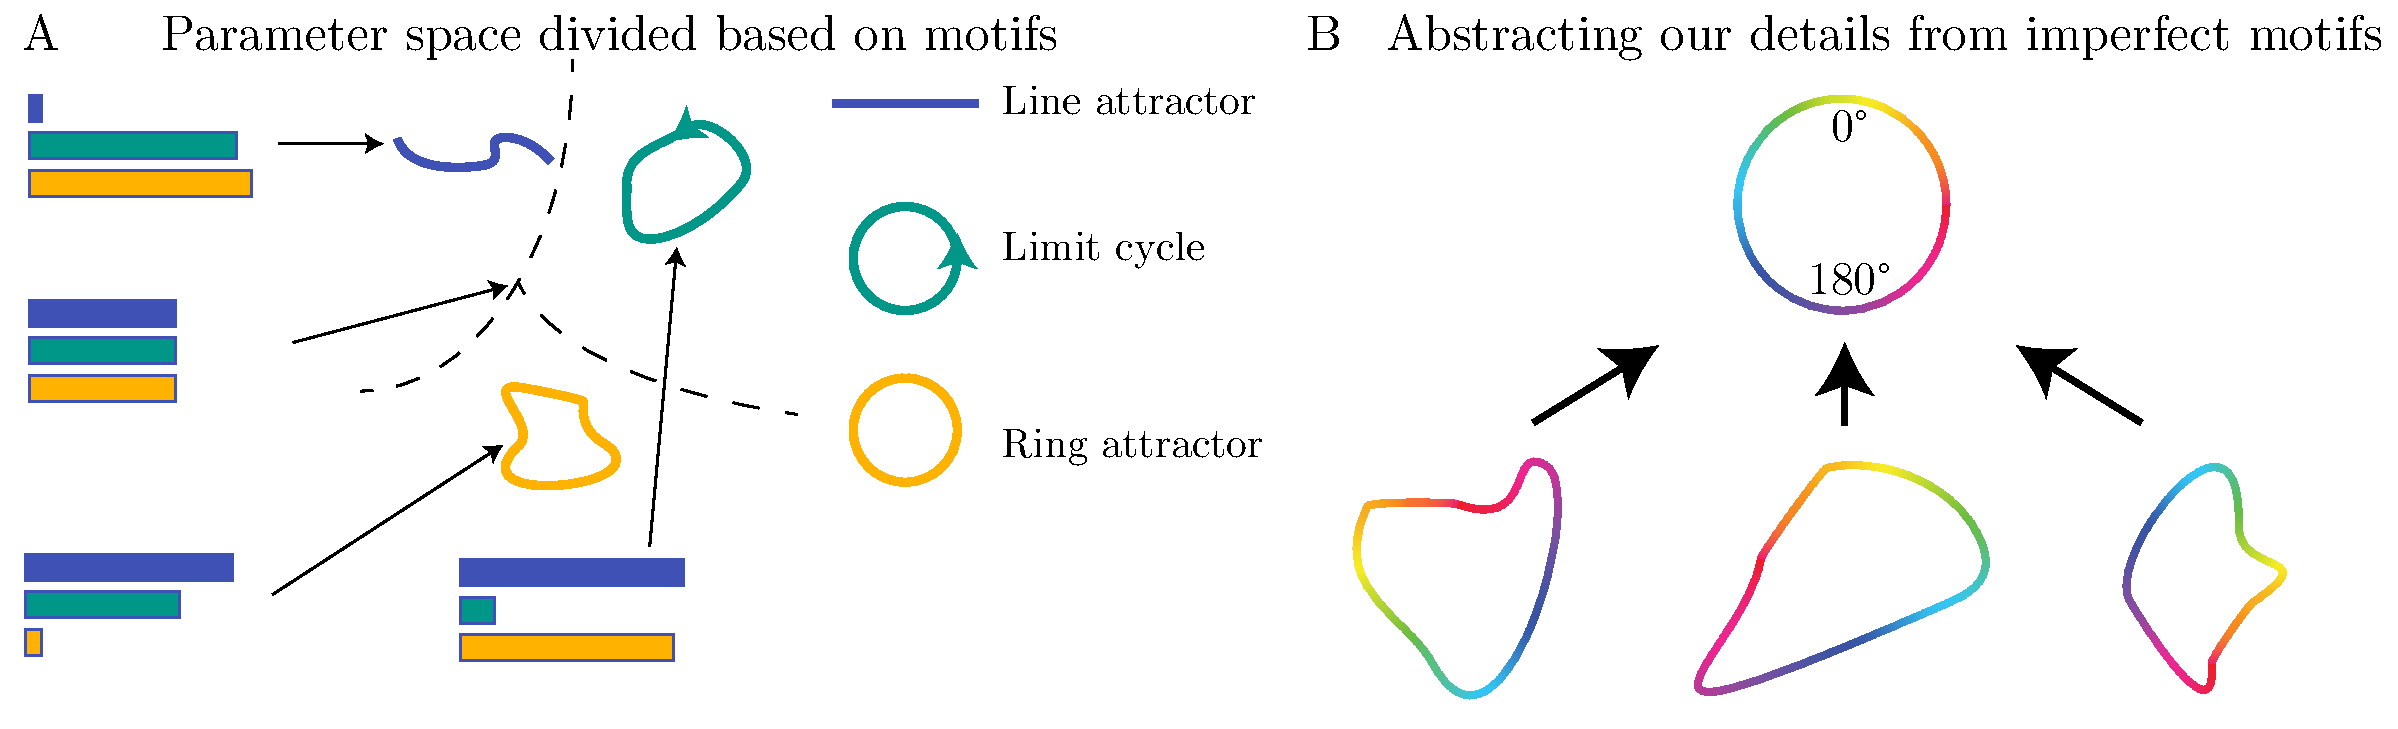
\includegraphics[width=\linewidth]{motifpspace_dssimilarity}
    \caption{Enlightening the space of theories with our dynamical motif torch.
    \textbf{(A)} Localizing a model in parameter space through dynamical motifs.
    \textbf{(B)} Abstracting out imperfections from an approximate ring attractor.
     }
    \label{fig:motifpspace_dssimilarity}
\end{figure}


\subsubsection{Motifs: The building blocks}
We use dynamical motifs as the fundamental building blocks of dynamical systems, capturing effective and interpretable behaviors such as approximate continuous attractors.
%simplification of BoA which simplify complex dynamics into stable basins in phase space 
These motifs are topologically distinct, meaning each represents a unique dynamical feature, ensuring clarity and avoiding redundancy.


%\subsubsection{The base case} % \subsubsection{Constructing}
% topological distinctness of the motifs

\paragraph{Enumerating attractors dimension-wise}
In dynamical systems, attractors can be systematically classified according to their topological dimension, with the simplest topological spaces serving as the fundamental building blocks at each level.
 This perspective provides a principled way to enumerate attractors that can arise in ordinary differential equations (ODEs).
\begin{enumerate}[start=0,label={\bfseries Dim \arabic*:}]
\item  Stable fixed point
\item  Bounded line attractor ($[0,1]\subset\reals$), ring attractor ($S_0^1$), stable limit cycle ($S_1^1$)
\item Plane attractor ($[0,1]^2$), Cylinder attractor ($[0,1]\times S_0^1$), Cylinder-LC attractor ($[0,1]\times S_1^1$), Torus attractor ($(S_0^1)^2$), Torus-LC attractor ($S_0^1\times S_1^1$), QPTA ($(S_1^1)^2$), Sphere attractor $S^2$
%\item ...
\end{enumerate}
This pattern continues, with higher-dimensional attractors constructed from fundamental topological spaces such as $S^n$ or their Cartesian and toroidal products.

%\ascomment{do we need to account for the possible existence of an attractor of the form $[0,1]^2\setminus D_{1/2}$? It won't affect the loss! So not for now!}

%what about higher dims??
extrinsic and intrinsic dimensionality\citep{jazayeri2021interpreting}
%low-dim neural activity

%\paragraph{Manifold decomposition}
%Triangulation


\subsubsection{An interpretable motif-centered comparison for dynamical systems}\label{sec:aut_motif_metric}
Building upon the dissimilarity measure defined earlier, we extend it to compare a target dynamical system with a library of motifs. Let \( f \in C^1 \) represent the vector field of the target system, and let \( g_i \) be a motif from the library. We assume the existence of a perturbation \( p \in C^1 \) and a homeomorphism \( \Phi: \mathbb{R}^n \rightarrow \mathbb{R}^n \) such that the perturbed system \( f + p \) can be aligned with the flow of \( g_i \) under \( \Phi \). 

The dissimilarity between \( f \) and each motif \( g_i \) is defined as the minimal perturbation \( p \) that satisfies this alignment, expressed as \( d(f, g_i) = \inf \|p\| \).
This allows us to projects the target system onto the motif library, producing a vector of distances to each motif.

%intuition
Convergence during training of RNNs: for tasks that rely on analog memory, the system's trajectory should exhibit a low dissimilarity to a dynamical motif that is a continuous attractor diffeomorphic to the memory manifold.
 This ensures that the system's behavior remains close to a well-defined dynamical motif, facilitating stable memory retrieval and task performance.


\subsubsection{Single global attractor}
We consider a target dynamical system $\dot{x} = f(x)$ which has a single global attractor.
 We assume that this system is topologically equivalent to one of a family of attractor motifs defined by dynamical systems $\dot{y} = g_i(y)$ where each $g_i$ represents a different canonical attractor in its normal form.
  This means that there exists a homeomorphism $\Phi$ mapping solutions of $g_i$ to solutions of $f$.
  Assuming smoothness, we model $\Phi$ as a diffeomorphism.
Our goal is to determine both the correct (best fitting/most explanatory) attractor motif $g_i$ and the diffeomorphism $\Phi$ given only observed trajectories $\{x_j(t_k)\}$ sampled from $f$.


\subsubsection{Trajectory based loss function}
Since we do not have direct access to the vector field but only to sampled trajectories, we approximate the system using a learned diffeomorphism \( \hat{\Phi}_\theta \), parameterized by a a Neural ODE (NODE) \citep{chen2018neural} (for other implementations, see Supp.Sec.~\ref{sec:architectures}).
% normalizing flow\citep{kobyzev2020normalizing,papamakarios2021normalizing}, an invertible ResNet\citep{he2016deep}
 We seek to minimize the discrepancy between the transformed trajectory and the corresponding trajectory in one of the candidate motifs.

%time repraram%
For the correct motif \( g_i \)  (satisfying orbit equivalence), there exists a reparametrization of time \( \tau(t) \) such that \(y(\tau(t)) \approx x(t)\)
with a trajectory \( y(t) \)  obtained by integrating \( \dot{y} = g_i(y) \) from an initial condition \( y(0) \). 
%So there exists $\mu(x)$ positive such that 
%We simplify this by assuming symmetry across space $\mu\in\reals_{>0}$.
A loss function capturing this trajectory discrepancy is given by:
\begin{equation}\label{eq:loss}
\mathcal{L}(\theta, \mu, i) = \sum_{t} \Big\| (x_k(t)) - \Phi_\theta(y_k(t)) \Big\|^2,
\end{equation}
where the trajectories \(y_k(t) \) are computed via numerical integration of \(\dot y =  g_i(y) \) from an initial condition $\hat y_k(0) = \Phi_\theta^{-1}(x_k(0))$. %add scaling by mu?
%The final optimization objective is:
%\[
%\min_{\theta, \mu,  i} \mathcal{L}(\theta, \mu, i). % + \lambda \mathcal{R}(\Phi_\theta), %regularization? NODE\citep{finlay2020trainnode}
%\]
%where \( \lambda \) is a regularization coefficient.
This formulation allows for the joint identification of both the correct motif \( g_i \) and the transformation \( \Phi \) that maps the observed system into its canonical form.


%intuition
Embedding ring attractors \citep{chaudhuri2019attractor}\citep{Sagodi2024a}

\subsubsection{Extensions to the canonical motifs}
\paragraph{Noisy motifs}
We consider noisy versions of motif trajectories governed by stochastic differential equations (SDEs) of the form
\begin{equation}
\dot x = g_i(x) + \sigma \, dW_t,
\end{equation}
where \( g_i(x) \) denotes the deterministic dynamics of the \( i \)-th motif, \( \sigma \) controls the noise amplitude, and \( W_t \) is a standard Wiener process.
To stabilize the trajectory alignment or improve optimization in the presence of noise, we incorporate simulated annealing by gradually decreasing \( \sigma \) over time.


\paragraph{Parameterized motifs}
We consider parameterized versions of motifs that involve adding to on- or rescaling the vector field both on- and off-manifold.
As an example, consider the stable limit cycle, which can be described by two scalar parameters: \( v \) and \( \alpha < 0 \).
The dynamics are given by:
\begin{equation}
\dot{r} = \alpha r (r - 1), %r_0?
\quad \dot{\theta} = v
\end{equation}
where \( r \) represents the radial coordinate and \( \theta \) the angular coordinate. Here, \( v \) controls the angular velocity, and \( \alpha \) determines the dynamics of the radial direction, where the system exhibits stable behavior at \( r = 1 \). This formulation allows for exploration of the effects of rescaling on the stability and behavior of the system, both in the radial and angular components of the phase space.


%justifications:
Biases on slow ring manifold for memory maintenance of circular values \citep{panichello2019error}.

%limitation: complexity of NN for VF
%but with noise we can not see too much detail 

%issue: overlap between motif spaces!


\subsubsection{The complexity of the homeomorphism}
To assess how much a learned homeomorphism $\Phi$ deforms space, we distinguish between a set of canonical transformation types, such as translations, permutations, rotations, uniform and non-uniform scalings (of space), and rescaling of the vector field (which affects global speed).
 While these operations are useful for interpreting specific deformation modes, they are not directly included in our complexity measure.
Instead, we capture the full, potentially nonlinear deformation induced by $\Phi$ by evaluating how much it deviates locally from the identity map. This is quantified using the Jacobian:
\begin{equation}
\left\|\frac{\partial \Phi}{\partial x} - \mathbb{I}\right\|
\end{equation}
which captures how much the local linear behavior of $\Phi$ differs from that of the identity transformation.
The norm of this deviation is computed either using the Frobenius norm or the spectral norm.
Finally, the \( L^p \) norm of the batch of Jacobians is computed, providing a scalar value that quantifies the overall local deformation across the space. A norm close to zero indicates that the transformation is nearly identity, while higher values suggest more significant deformations.

%measure-preserving (Hamiltonian) transformation

\paragraph{Wasserstein distance between the distribution over trajectories}
\citep{bion2019wasserstein}
The Wasserstein distance evaluates how these local distortions aggregate over the distribution of trajectories.
The Jacobian norm relates to the Wasserstein distance by capturing local distortions that contribute to the global changes in the distribution, which are reflected in the Wasserstein distance between the trajectories' distributions.


%\subsection{Demonstration}
%We illustrate the application of our method on a simple example in Figure~\ref{fig:all_motifs_vdp}, where different motifs from the library are fitted to noisy trajectories generated by a Van der Pol oscillator.
%Observe that the limit cycle motif provides the best fit, capturing the underlying oscillatory dynamics more accurately than the alternatives.





\subsection{Reducing the dimensionality} % to a minimal dimensional motif
\subsubsection{Homeomorphism from minimal dimensional motif}
Let \( f \in C^1 \) define the vector field of a target dynamical system on \( \mathbb{R}^n \), and let \( g_i \in C^1(\mathbb{R}^m, \mathbb{R}^m) \) be a dynamical motif of minimal dimension \( m \leq n \) that captures the essential dynamics of \( f \). Then there exists a perturbation \( p \in C^1(\mathbb{R}^n, \mathbb{R}^n) \) and a homeomorphism \( \Phi: \mathbb{R}^m \to \mathbb{R}^n \) such that the flow \( \psi_{f+p} \) of the perturbed system is topologically conjugate to the embedded flow \( \Phi \circ \psi_{g_i} \). %, i.e.,
%\begin{equation}\label{eq:hom_from_motif}
%\|\psi_{f+p} - \Phi \circ \psi_{g_i} \|_\infty = 0.
%\end{equation}


\subsubsection{Surjective mapping to minimal dimensional motif}
Let \( f \in C^1(\mathbb{R}^n, \mathbb{R}^n) \) define the vector field of a target dynamical system, and let \( g_i \in C^1(\mathbb{R}^m, \mathbb{R}^m) \) be a dynamical motif of minimal dimension \( m \leq n \) that captures the essential dynamics of \( f \). Then there exists a perturbation \( p \in C^1(\mathbb{R}^n, \mathbb{R}^n) \) and a surjective continuous map \( \Phi: \mathbb{R}^n \to \mathbb{R}^m \) such that the flow \( \psi_{g_i} \) of the motif is semi-conjugate to the flow \( \psi_{f+p} \) of the perturbed system via \( \Phi \). %, i.e.,
%\begin{equation}\label{eq:perfect_motif_fit}
%\| \psi_{g_i} - \Phi \circ \psi_{f+p} \|_\infty = 0.
%\end{equation}


Problem: trivial solution $\Phi(x) = 0$ for $x\in\mathcal{D}$.\\
Solution (?): injectivity per orbit (still allow for non-injectivity across orbits)




%%%%%%%%%%%%%%%%%
\section{Results}
An imperfect ring attractor: Sec.~\ref{sec:imp_ring}

A noisy target: Sec.~\ref{sec:noisy}

Compared methods: Sec.~\ref{sec:compare_method}

Demonstration: Sec.~\ref{sec:target_demonstrations}

\subsection{Finding the deformation to a ring attractor}\label{sec:imp_ring}
%justification of this  experiment

%description

%interpretation of results
Fig.~\ref{fig:ring_pert_fig}

\begin{figure}[htbp]
    \centering
    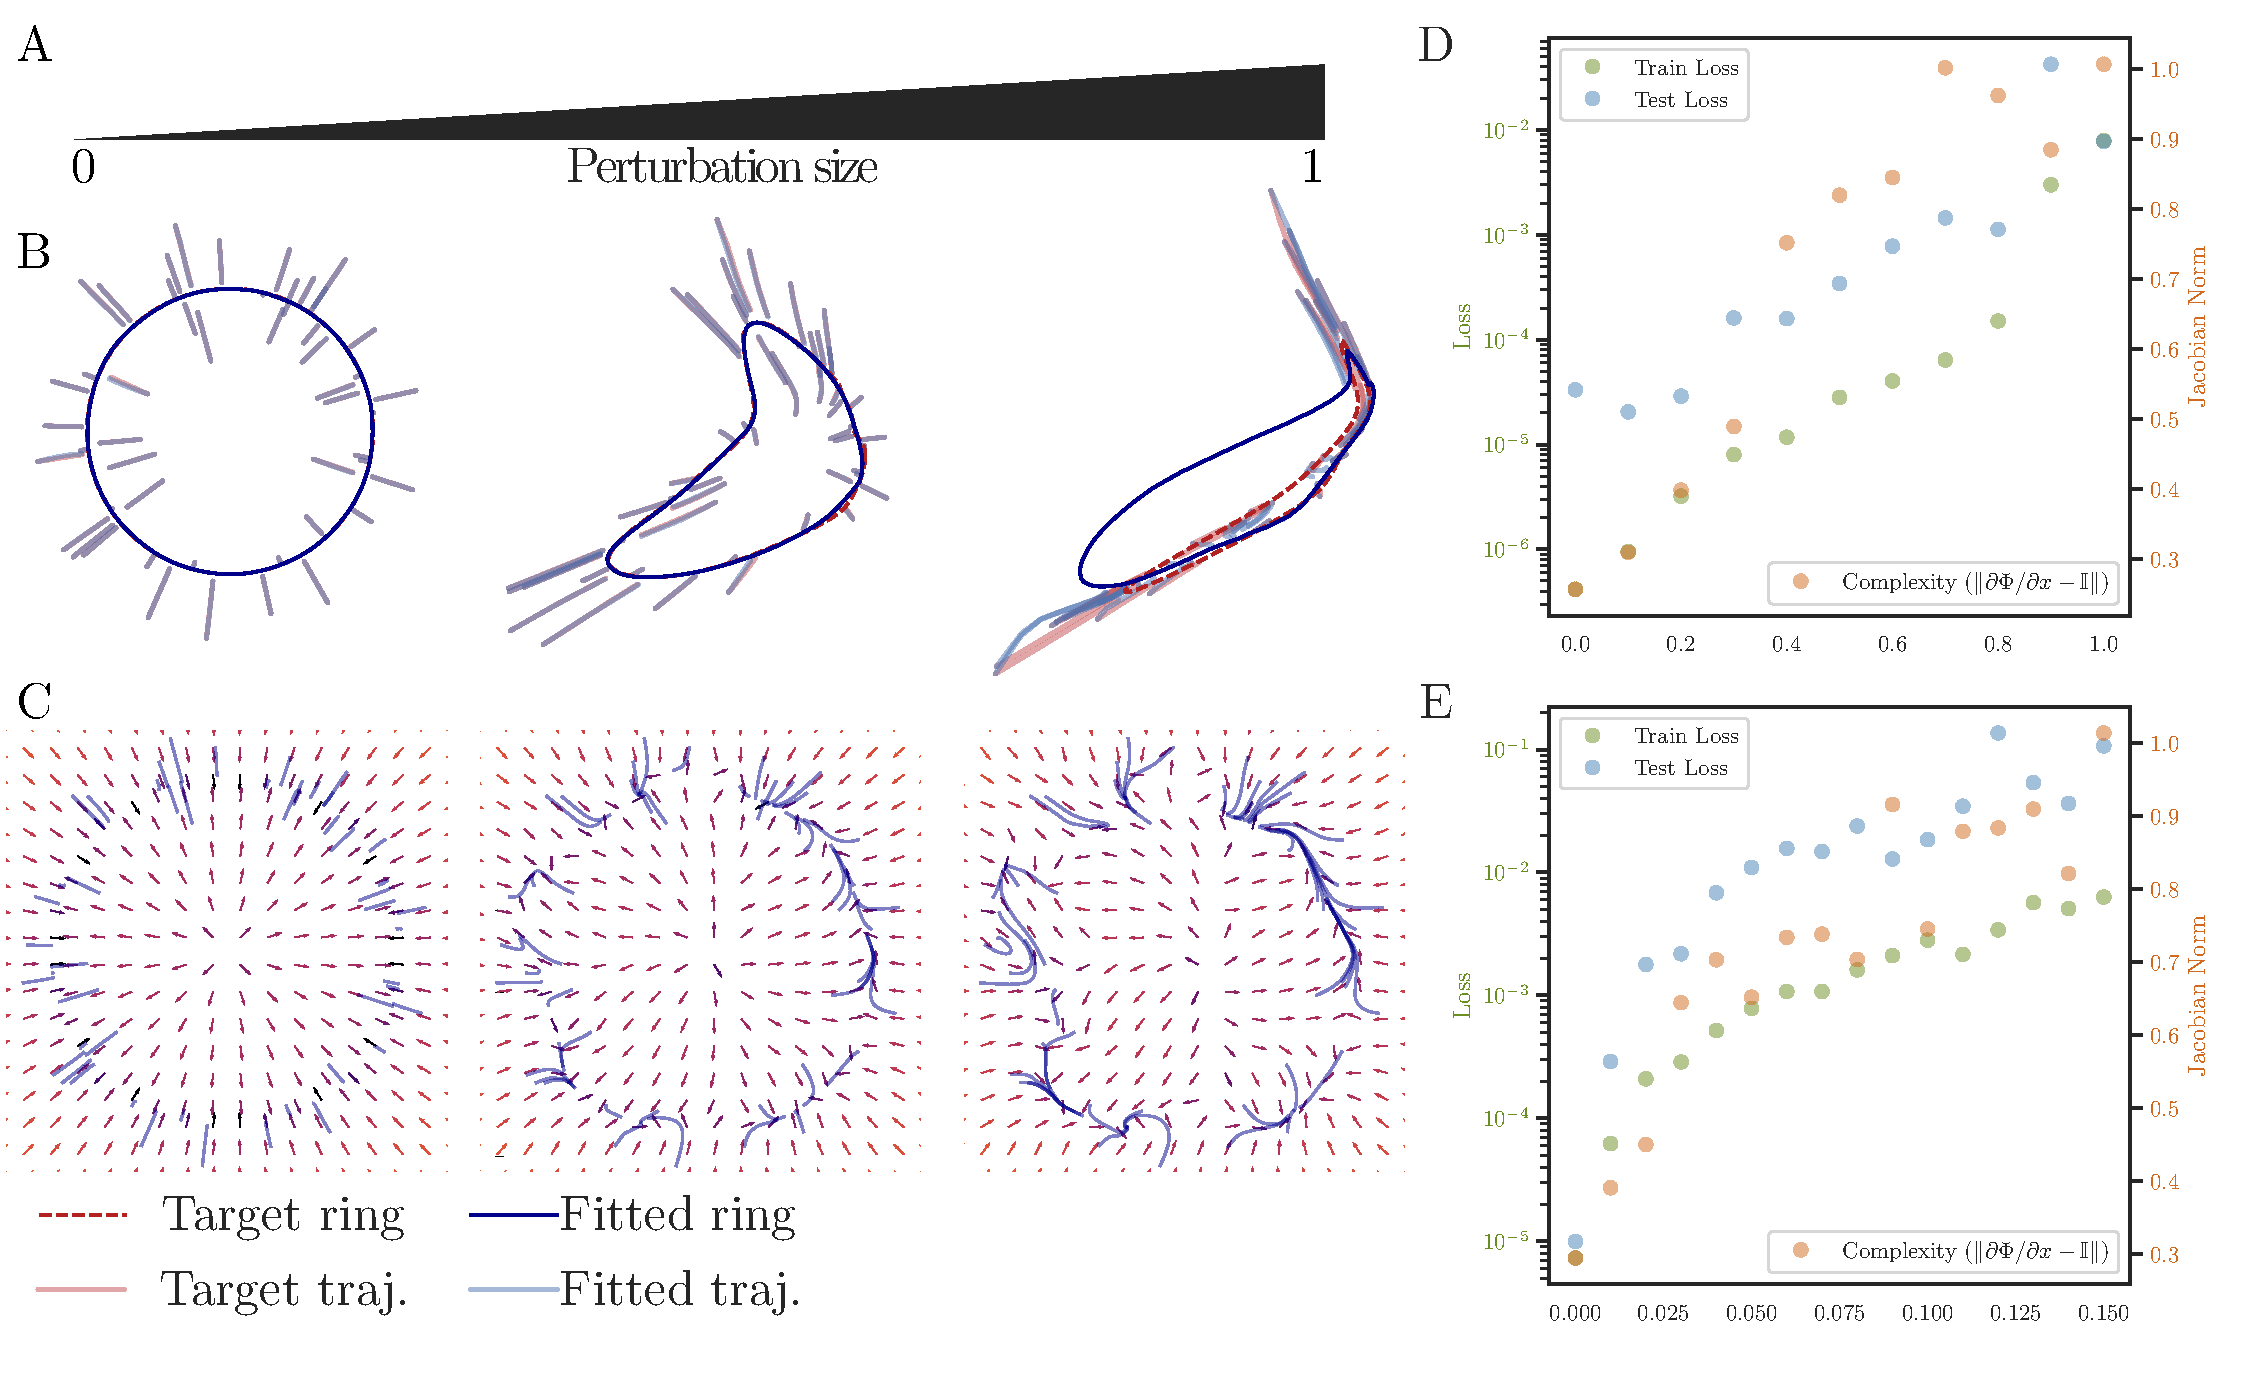
\includegraphics[width=.9\linewidth]{ring_pert_fig}
    \caption{Finding deformed ring attractors. 
    (\textbf{A}) We consider two types of perturbations to a ring attractor that are controlled by a scalar perturbation size.
    (\textbf{B}) The first type considers a perturbation that leaves the continuum of fixed points intact: it merely deforms the ring attractor and the transient orbits but the perturbed system is still topologically conjugate to the original.
    (\textbf{C}) The second type is a perturbation to the vector field. 
    }
    \label{fig:ring_pert_fig}
\end{figure}

\subsection{A noisy target}\label{sec:noisy}

\subsection{Comparison to other methods}\label{sec:compare_method}

\paragraph{DSA}%https://github.com/mitchellostrow/DSA
metric: DSA score

%\paragraph{Phase2Vec} %https://github.com/nomoriel/phase2vec

%\paragraph{DFORM} %NO CODE????

\paragraph{SPE} %https://github.com/nitzanlab/prototype-equivalences
Smooth prototype equivalences (SPE) is a method that fits a diffeomorphism from the given data to normal forms \citep{friedman2025characterizing}.
However, their method is dependent on knowledge of the vector field of the target system.
Furthermore, they have only considered limit cycle versus fixed point dynamics for their library.
metric: cycle-error

%\paragraph{SSMLearn} %https://github.com/haller-group/SSMLearnPy/tree/main

% \paragraph{MARBLE}
%MARBLE \citep{gosztolai2025marble} proposes a similarity measure based on local vector field features (vectors and higher-order derivatives) sampled from across the phase space.
% The features are embedded into lower-dimensional space through contrastive learning, and the embedded distributions from different systems can be compared using an optimal transport distance.

%\subsubsection{Comparison to DSA and SPE}
\begin{figure}[htbp]
    \centering
    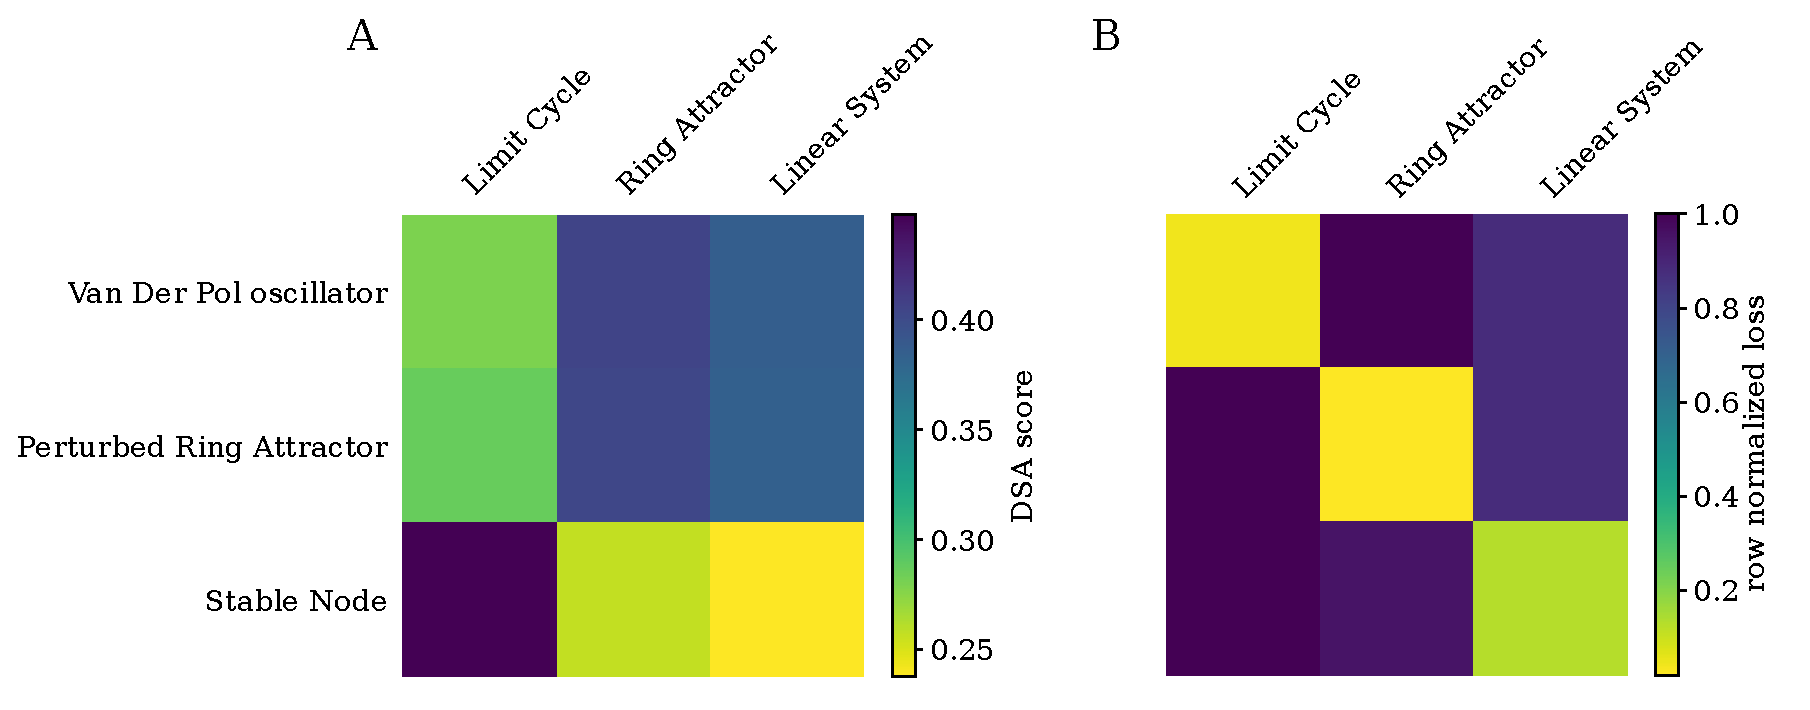
\includegraphics[width=0.75\linewidth]{dsa_vs_mbs}
    \caption{DSA vs Motif Based Similarity.}
    \label{fig:ds_vs_mbs}
\end{figure}

\subsection{Many target systems}\label{sec:target_demonstrations}
Supp.Sec.~\ref{sec:target_systems}





%%%%%%%%%%%%%%%%%
\section{Discussion}

\subsection{Limitations}
Assumption: the invariant set of the target needs to be well-sampled.


\subsection{}
Limits to neuroscientific understanding \citep{chirimuuta2024brain}


simplest isn't always the best \citep{dyer2023simplest}


planning: complex dynamical motifs that correspond to current and future actions \citep{vyas2020ctd}


\newpage
\bibliographystyle{unsrtnat_IMP_v1}
\bibliography{../all_ref.bib,../catniplab.bib}


\newpage
\appendix


%%%%%TOP
\section{Topology}\label{sec:topology}

\subsection{Approximating homeomorphisms}\label{sec:homeomorphisms}


Any homeomorphism on a $p$-dimensional Euclidean space can be approximated by a Neural ODE or an i-ResNet operating on a $2p$-dimensional Euclidean space \citep{zhang2020approximation}.

Capping a Neural ODE or an i-ResNet with a single linear layer is sufficient to turn the model into a universal approximator for non-invertible continuous functions \citep{zhang2020approximation}.

\subsubsection{Implementations}



\subsection{Approximating diffeomorphisms}\label{sec:diffeomorphisms}
%any homeomorphism on a $p$-dimensional Euclidean space can be approximated by a Neural ODE or an i-ResNet operating on a $2p$-dimensional Euclidean space \citep{zhang2020approximation}
Any homeomorphism of $\mathbb {R} ^{n}$ can be approximated by a neural ODE operating on $\mathbb {R} ^{2n+1}$, proved by combining Whitney embedding theorem for manifolds and the universal approximation theorem for neural networks  \citep{zhang2020approximation}.

%diffeomorphisms from gradient information of desired costs \citep{lai2021parallelised}

\subsubsection{Flow-based}
\paragraph{Neural ODEs}
Neural ODEs \citep{chen2018neural} represent the latest instance of continuous deep learning model for time series, first developed in the context of continuous recurrent networks \citep{cohen1983absolute}.
%
Neural ODEs model the continuous trajectory of the hidden state \( \mathbf{h}(t) \) as the solution to an ordinary differential equation parameterized by a neural network. Mathematically, the dynamics are defined by:

\[
\frac{d \mathbf{h}(t)}{dt} = f(\mathbf{h}(t), t, \theta)
\]

where \( \mathbf{h}(t) \) is the hidden state at time \( t \), \( f \) is a neural network with parameters \( \theta \), and \( t \) represents time. Given an initial condition \( \mathbf{h}(t_0) = \mathbf{h}_0 \), the evolution of the hidden state over time is computed by solving the ODE using numerical solvers, allowing the model to capture complex, continuous transformations.

%example of f
\textbf{Fully Connected Neural Network (Feedforward Network)}:

\[
f(\mathbf{h}(t), t, \theta) = W_2 \sigma(W_1 \mathbf{h}(t) + \mathbf{b}_1) + \mathbf{b}_2
\]

Here, \( \sigma \) is an activation function (e.g., ReLU, tanh, or sigmoid), \( W_1, W_2 \) are weight matrices, and \( \mathbf{b}_1, \mathbf{b}_2 \) are bias vectors.
 This form models the ODE dynamics using a simple two-layer feedforward network.

Universal approximation properties of neural operator architectures \citep{lu2021learning, kissas2022learning, kovachki2021universal}.

NODE\citep{finlay2020trainnode}
\citep{torchdiffeq}


\paragraph{Applications}
%NODEs in neuroscience%
Neural ordinary differential equations (NODEs) are being increasingly adopted in computational and systems neuroscience, showing improved performance compared to current approaches \citep{kim2021inferring,geenjaar2023learning,sedler2023expressive,elgazzar2024universal,rubanova2019latent,coelho2024enhancing}.



\subsubsection{Invertible ResNets}
the layers of a ResNet can be considered as Euler-discretization of the integration of a flow of a diffeomorphism\citep{rousseau2020residual}






% Normalizing flows\citep{kobyzev2020normalizing}

Conjugate Mappings \citep{bramburger2021conjugate}


\subsubsection{Decomposing diffeomorphisms}\label{sec:diff_dec}
\paragraph{Lie}
Since diffeomorphisms form a Lie group under composition, a diffeomorphism 
\( f \) can be written formally as:
\[
f = \exp(X),
\]
where \( X \) is a vector field (i.e., an element of the Lie algebra of the diffeomorphism group). Expanding \( X \) in a Fourier basis:
\[
X(x) = \sum_k \hat{X}(k) e^{i k \cdot x}
\]
provides a Fourier-like decomposition of the infinitesimal generator.

\paragraph{}
A simple sufficient condition for a family of flows on a smooth compact manifold $M$ to generate the group $\Diff0_(M)$ of all diffeomorphisms of $M$ that are isotopic to the identity \citep{caponigro2010families}.

Stability of diffeomorphisms implies that $\Diff(M)\subset C^1(M,M)$  is an open subset.


\subsubsection{Implementations}
Freia\citep{freia} %https://github.com/vislearn/FrEIA
Torchdiffeq: \citep{torchdiffeq}
NF\citep{dinh2016density} % https://github.com/AxelNathanson/pytorch-normalizing-flows?tab=readme-ov-file
\citep{stimper2023normflows} % https://github.com/VincentStimper/normalizing-flows



\subsubsection{Jacobian of homeomorphism}
 For a smooth homeomorphism \( \Phi \), the Jacobian \( J_{\Phi}(x) \in \mathbb{R}^{n \times n} \) is the matrix of partial derivatives:
\[
J_{\Phi}(x) = \left[ \frac{\partial \Phi_i}{\partial x_j}(x) \right]_{i,j}.
\]

\paragraph{Matrix norm of the Jacobian at a point \( x \).} Typically, we use either the operator norm (e.g., induced 2-norm) or the Frobenius norm:
\[
\|J_{\Phi}(x)\| :=
\begin{cases}
\|J_{\Phi}(x)\|_2 & \text{(spectral/operator norm)} \\
\|J_{\Phi}(x)\|_F = \left( \sum_{i,j} \left| \frac{\partial \Phi_i}{\partial x_j}(x) \right|^2 \right)^{1/2} & \text{(Frobenius norm)}.
\end{cases}
\]

\paragraph{Norm of Jacobian at a point \( x \) minus the identity.}
\(\|J_{\Phi}(x) - \mathbb{I}\| \)

\paragraph{Operator \( L^p \) norm of the Jacobian over a domain \( \Omega \subseteq \mathbb{R}^n \), with respect to a measure \( \mu \):}
\[
\|J_{\Phi}\|_{L^p(\mu)} = \left( \int_{\Omega} \|J_{\Phi}(x)\|^p \, d\mu(x) \right)^{1/p}.
\]



\newpage
\section{Geometry}
Geometric Learning on Manifolds\citep{mostowsky2024geometrickernels}


\paragraph{Standard Matérn Kernel (Based on Geodesic Distance)}
Replace the Euclidean distance  $\| x - x' \|$  in the Matérn kernel with the distance to the manifold  $ d_{\text{manifold}}(x, x')$. 
This distance is now the measure of how far two points are from each other, but considering the geometry of the manifold.
\begin{equation}
k(x, x') = \frac{1}{\Gamma(\nu)} \left( \frac{\sqrt{2\nu} d_{\text{manifold}}(x, x')}{\ell} \right)^\nu K_\nu\left( \frac{\sqrt{2\nu} d_{\text{manifold}}(x, x')}{\ell} \right).
\end{equation}


\subsection{Implementations}
\citep{miolane2020geomstats}
%https://github.com/geomstats/geomstats?tab=readme-ov-file







%%%%%DS
\newpage
\section{Dynamical systems background}

\subsection{Comparing dynamics}
Binary/Discrete: equivalence

Continuous comparison: metric/distance/dissimilarity



\subsubsection{Exact equivalence: Topological conjugacy}\label{sec:top_conj}

Topological conjugacy is an equivalence relation on the category of flows. %Behavioral space
\begin{definition}[Topological conjugacy]\label{def:top_conj}
let $\phi$ be a flow on $X$, and $\psi$ a flow on $Y$, with $X$, $Y$, and $h\colon Y \to X$ as above.

We say that $\phi$ is \emph{topologically semiconjugate} to $\psi$ if, by definition, $h$ is a surjection such that
\[
\phi(h(y), t) = h \circ \psi(y, t), \quad \text{for all } y \in Y, \; t \in \mathbb{R}.
\]
Furthermore, $\phi$ and $\psi$ are said to be \emph{topologically conjugate} if they are topologically semiconjugate and $h$ is a homeomorphism.
\end{definition}

Smooth equivalence is an equivalence relation in the category of smooth manifolds with vector fields. %model space
\begin{definition}[Smooth equivalence]\label{def:smooth_equivalence}
Two dynamical systems defined by the differential equations 
\[
\dot{x} = f(x) \quad \text{and} \quad \dot{y} = g(y)
\]
are said to be \emph{smoothly equivalent} if there exists a diffeomorphism \( h \colon X \to Y \) such that
\[
f(x) = M^{-1}(x) \, g(h(x)) \quad \text{where} \quad M(x) = \frac{d h(x)}{d x}.
\]
In that case, the dynamical systems can be transformed into each other by the coordinate transformation \( y = h(x) \).
\end{definition}

\begin{definition}[Orbital equivalence]
Two dynamical systems on the same state space, defined by 
\[
\dot{x} = f(x) \quad \text{and} \quad \dot{x} = g(x),
\]
are said to be \emph{orbitally equivalent} if there exists a positive function \( \mu \colon X \to \mathbb{R} \) such that
\[
g(x) = \mu(x) f(x).
\]
\end{definition}
Orbitally equivalent systems differ only in their time parametrization.


\subsection{}
Two dynamical systems on the same state space:
\[
\dot{x} = f(x) \quad \text{and} \quad \dot{x} = g(x).
\]

Let 
\begin{itemize}
\item $p\in C^1$
\item $\Phi$ a homeomorphism
\item $\mu\colon \reals^n\rightarrow \reals$ positive function
\end{itemize}
such that 
\begin{enumerate}
\item $\psi_{\mu \cdot (f+p)}$ is topologically conjugate to $\psi_{g}$
\item Take $\inf_p \|p\|$, $\inf_\mu \|\mu\|$, $\inf_\Phi \|\Phi\|$
%\item $f(x) = \mu(x) D\Phi(x)^{-1}(x) \, g(h(x))$ % is topologically conjugate
\end{enumerate}

%\begin{definition}\label{def:top_conj}
%Let \( f: X \to X \) and \( g: Y \to Y \) be two continuous dynamical systems, where \( X \) and \( Y \) are topological spaces.
% The systems are said to be \emph{topologically conjugate} if there exists a homeomorphism \( h: X \to Y \) such that the following conjugacy condition holds:
%\[
%h \circ f = g \circ h.
%\]
%That is, the following diagram commutes:
%\begin{tikzcd}[row sep=large, column sep=large]
%X \arrow[r, "f"] \arrow[d, "h"'] & X \arrow[d, "h"] \\
%Y \arrow[r, "g"'] & Y
%\arrow[from=1-2, to=2-1, phantom, "\circlearrowleft", description, pos=0.5]
%\end{tikzcd}
%\end{definition}

\paragraph{Topological conjugacy of time series}
\citep{dlotko2024topconj}


\paragraph{Topological conjugacy on and off the invariant manifold}
Taking apart topological conjugacy (homeomorphism from motif):
\begin{itemize}
\item On asymptotic / $\omega$-limit set / invariant set
\item On transients \citep{koch2024biological}
\end{itemize}


\subsubsection{Defective equivalence: Mostly Conjugate Dynamical Systems}
\citep{skufca2007relaxing, skufca2008mostlyconjugate, bollt2010comparing}



\subsection{Normal forms}

\subsubsection{Normal forms for autonomous dynamics}%ISOLATED FPS
Examples
Saddle ring
\begin{equation}
\begin{aligned}
\dot{x} &= (\sqrt{x^2 + y^2} - 1) x, \\
\dot{y} &= (\sqrt{x^2 + y^2} - 1) y.
\end{aligned}
\end{equation}


\subsubsection{Beyond isolated fixed points}
How do we define a normal form when the system has a continuous attractor, such as a manifold of stable fixed points or limit cycles?

\paragraph{Limit cycles}%exists
Let 
\[
\dot{x} = f(x), \quad x \in \mathbb{R}^n,
\]
with a \emph{hyperbolic limit cycle} \( \gamma(t) \) of period \( T \), meaning:
\[
\gamma(t + T) = \gamma(t), \quad \dot{\gamma}(t) = f(\gamma(t)).
\]
The linearized dynamics transverse to the cycle have no Floquet multipliers on the unit circle except the trivial one corresponding to time shift.

Let \( x = \Phi(\theta, r) \), where: %Phi is a diffeom
\begin{itemize}
  \item \( \theta \in \mathbb{S}^1 \): phase variable (e.g., time along the cycle),
  \item \( r \in \mathbb{R}^{n-1} \): transverse coordinates.
\end{itemize}
In these coordinates, the system becomes:
\[
\begin{aligned}
\dot{\theta} &= 1 + a_1(r) + a_2(r) + \dots, \\
\dot{r} &= \Lambda(\theta) r + b_2(\theta, r) + b_3(\theta, r) + \dots,
\end{aligned}
\]
where \( \Lambda(\theta) \) is the linearized transverse dynamics (from Floquet theory),
and  \( a_k(r) \in \mathbb{R} \), \( b_k(\theta, r) \in \mathbb{R}^{n-1} \) are \( \mathcal{O}(\|r\|^k) \).
The system can be simplified via near-identity, time-periodic coordinate transformations (sometimes called Floquet–normal form reduction).

\textbf{Example: Van der Pol.} 
The Van der Pol oscillator is a system described by the equations:
\[
\dot{x}_1 = x_2, \quad \dot{x}_2 = \mu (1 - x_1^2) x_2 - x_1,
\]
where \( \mu \) is a nonlinearity parameter.

To analyze the limit cycle behavior, we use polar coordinates \( x_1 = r \cos(\theta) \) and \( x_2 = r \sin(\theta) \), where:
\[
\dot{r} = -\mu r + \mathcal{O}(r^2), \quad \dot{\theta} = 1 + \mathcal{O}(r).
\]
Thus, the normal form near the limit cycle is:
\[
\dot{\theta} = 1, \quad \dot{r} = -\mu r + \mathcal{O}(r^2),
\]
which describes a stable limit cycle with phase \( \theta \) evolving uniformly and radial contraction controlled by \( \mu \).


\paragraph{Continuous attractors}%our proposal
Let $\manifold\subset\reals^n$  be a smooth normally hyperbolic invariant manifold (NHIM).
A \emph{normal form} near a continuous attractor \(\manifold \subset \mathbb{R}^n \) is a change of coordinates 
\( x = \Phi(\theta, r) \), with:
\begin{itemize}
  \item \( \theta \in \mathbb{R}^d \): coordinates on the attractor \( \manifold\),
  \item \( r \in \mathbb{R}^{n-d} \): coordinates transverse to \(\manifold \),
\end{itemize}
such that the vector field becomes:
\[
\begin{aligned}
\dot{\theta} &= 0, \\
\dot{r} &= -\Lambda(\theta) r + \mathcal{O}(\|r\|^2),
\end{aligned}
\]
where \( \Lambda(\theta) \) is positive definite, ensuring contraction toward the attractor \(\manifold\).

Equivariant bifurcation theory provides normal forms that are invariant under group action


\paragraph{Translation to center around origin}




\subsection{Pushforward of the vector field: flow under a diffeomorphism}
See e.g., Eq.1.2 in \citep{agrachev2013control}.

Given a diffeomorphism \( \Phi: M \to M \), we consider the vector field \( V \in \text{Vec}(M) \), governing the dynamical system:
\[
\dot{q} = V(q).
\]

The diffeomorphism \( \Phi \) induces a pushforward of the vector field \( V \), given by:
\[
(\Phi_* V)(p) = D\Phi(\Phi^{-1}(p)) V(\Phi^{-1}(p)),
\]
where \( D\Phi \) is the differential (Jacobian) of \( \Phi \).  

\paragraph{Transformed Dynamical System}
In the new coordinates \( x = \Phi(q) \), differentiating with respect to time gives:
\[
\dot{x} = \frac{d}{dt} \Phi(q) = D\Phi(q) \dot{q}.
\]

Substituting \( \dot{q} = V(q) \), we obtain:
\[
\dot{x} = D\Phi(q) V(q).
\]

Rewriting in terms of \( x \), where \( q = \Phi^{-1}(x) \), the transformed vector field in the new coordinates is:
\[
\dot{x} = (D\Phi \circ \Phi^{-1}) V(\Phi^{-1}(x)).
\]

Thus, the transformed vector field is:
\[
V' = \Phi_* V = (D\Phi \circ \Phi^{-1}) \cdot (V \circ \Phi^{-1}).
\]
This describes how a diffeomorphism \( \Phi \) acts on the vector field governing the dynamics.




\subsubsection{Normal forms for input-driven dynamics}
Normal form representation of control systems  \citep{gilbert1963controllability}
Brunovsky normal form is a canonical form for controllable linear systems.



\subsection{Coherence in behavior}
\subsubsection{Perfect coherence: Invariant manifolds}%+forward invariance


\subsubsection{Asymptotic behavior}\label{sec:asymptotic}
Infinite time horizon perfect coherence





\subsubsection{Imperfect coherence}%+forward invariance
\paragraph{Almost invariant manifolds}
 Almost-invariant regions are identified via eigenvectors of a transfer operator and are ranked by the corresponding eigenvalues in the order of the sets' invariance or ``leakiness'' \citep{froyland2009almost}.
    
    
    
\paragraph{Metastable behavior}\label{sec:metastable}
   \citep{brinkman2022metastable}
    
    
\paragraph{Coherent regions}
Regions that remain coherent and relatively nondispersive over finite periods of time \citep{fackeldey2019metastable}.



%\subsection{Reconstructing dynamics}\label{sec:rec_dyn}
%\subsubsection{NODE}
%\citep{finlay2020trainnode}



\newpage
%\section{Dynamical systems contributions}
%Overview  

\section{Generalizing motif metric to input-driven systems}
We generalize the idea of autonomous attractors (Sec.~\ref{sec:aut_motif_metric}) for input-driven systems.

Let the target system be
\[
\dot{x} = f(x) + g(u, x),
\]
where \( g(u, x) \in C^1 \) captures the input-driven dynamics.

Let \( \{ g_i(x) \} \) be a fixed set of motif vector fields defining a canonical control-affine structure (see Supp.Sec.~\ref{sec:attaction}):
\[
g_{\text{affine}}(u, x) := \sum_i u_i g_i(x).
\]

We define the distance between the true input dynamics and the control-affine approximation as
\[
d(g(u, x), \{ g_i(x) \}) := \inf_{\{ g_i \}} \left\| g(u, x) - \sum_i u_i g_i(x) \right\|_{\mathcal{U}, \infty},
\]
where the norm \( \| \cdot \|_{\mathcal{U}, \infty} \) is taken over a compact domain \( \mathcal{U} \times \mathcal{X} \subset \mathbb{R}^m \times \mathbb{R}^n \), and the infimum may be constrained to a motif class.

This distance quantifies the degree to which the system's input-driven dynamics can be expressed as a linear combination of the motif vector fields.

\section{The action of the input on the attractor manifold}\label{sec:attaction}
For stationary attractors (continuous attractors), the control-affine framework characterizes the simplest way to describe the action of the input (see Supp.Sec.~\ref{sec:statattaction}).
For periodic attractors, the action needs to be defined in terms of the phase resetting curve (see Supp.Sec.~\ref{sec:perattaction}).


\subsection{Action of the input on  stationary attractors}\label{sec:statattaction}
\subsubsection{Control-affine}\label{sec:controlaffine}
Let the system evolve according to the control-affine dynamics:
\[
\dot{x}(t) = f(x(t)) + \sum_{i=1}^m u_i(t) g_i(x(t)),
\]
where \( x(t) \in \mathbb{R}^n \) is the state, \( u(t) \in \mathbb{R}^m \) is the input, \( f : \mathbb{R}^n \to \mathbb{R}^n \) governs the autonomous dynamics, and \( g_i : \mathbb{R}^n \to \mathbb{R}^n \) are the input vector fields.

Suppose the system admits a manifold \( \mathcal{M} \subset \mathbb{R}^n \) of fixed points under the autonomous dynamics:
\[
\mathcal{M} = \{ x \in \mathbb{R}^n \mid f(x) = 0 \}.
\]
We assume that each input vector field \( g_i \) is tangent to the manifold at every point:
\[
g_i(x) \in T_x \mathcal{M}, \quad \forall x \in \mathcal{M}, \quad i = 1, \dots, m.
\]
Define \( \mathfrak{g}_x = \operatorname{span} \{ g_1(x), \dots, g_m(x) \} \subset T_x \mathcal{M} \) to be the subspace of directions accessible by the inputs at state \( x \in \mathcal{M} \). Let \( \mathcal{L}_x \) denote the Lie algebra generated by \( \{g_1, \dots, g_m\} \) under the Lie bracket of vector fields, evaluated at \( x \):
\[
\mathcal{L}_x = \operatorname{span} \left\{ Y(x) \,\middle|\, Y \in \mathrm{Lie}(g_1, \dots, g_m) \right\}.
\]
Since the Lie brackets of tangent vector fields remain tangent, it follows that \( \mathcal{L}_x \subseteq T_x \mathcal{M} \) for all \( x \in \mathcal{M} \).
Thus, the integral manifolds generated by the Lie algebra \( \mathrm{Lie}(g_1, \dots, g_m) \) are contained in \( \mathcal{M} \), and describe the directions along which the state can be moved by time-varying inputs:
\[
\mathcal{O}(x) = \left\{ \phi_{t_k}^{Y_k} \circ \cdots \circ \phi_{t_1}^{Y_1}(x) \,\middle|\, Y_j \in \mathrm{Lie}(g_1, \dots, g_m),\ t_j \in \mathbb{R} \right\} \subseteq \mathcal{M},
\]
where \( \phi_t^Y \) denotes the flow of the vector field \( Y \) at time \( t \). In this sense, the input acts as a generator of motion along the manifold \( \mathcal{M} \) via the action of the associated Lie algebra.


\subsubsection{Non-Affine Case}\label{sec:controlaffine}
Linearize!

Assuming smoothness, we expand the input-driven dynamics \( F(x, u) \) in a Taylor series around \( u = 0 \):
\[
F(x, u) = f(x) + \sum_{i} u_i g_i(x) + \sum_{i,j} u_i u_j h_{ij}(x) + \cdots,
\]
where
\begin{align}
f(x) &= F(x, 0),\\
g_i(x) &= \left. \frac{\partial F}{\partial u_i}(x, u) \right|_{u = 0},\\
h_{ij}(x) &= \left. \frac{1}{2} \frac{\partial^2 F}{\partial u_i \partial u_j}(x, u) \right|_{u = 0}.
\end{align}

Here, \( \{g_i(x)\} \) represents the first-order (linear) influence of the inputs on the dynamics, corresponding to the control-affine approximation. The higher-order terms \( h_{ij}(x) \) and beyond capture nonlinear interactions between input components and their influence on state evolution.


%v-equation and r-equation \citep{miller2012mathematical}
\paragraph{Voltage rate} %easy!
Consider the continuous-time RNN dynamics:
\[
\dot{x} = F(x, u) = -x + W\phi(x) + B u,
\]
where \( x \in \mathbb{R}^n \) is the state, \( u \in \mathbb{R}^m \) is the input, \( W \in \mathbb{R}^{n \times n} \) is the recurrent weight matrix, \( B \in \mathbb{R}^{n \times m} \) is the input weight matrix, and \( \phi : \mathbb{R}^n \to \mathbb{R}^n \) is a smooth nonlinearity applied elementwise.
Then, $g_i(x) = B_i$, where \( B_i \) denotes the \( i \)-th column of \( B \).

Since the \( g_i \) are constant vector fields, the control vector fields are automatically tangent to \( \mathcal{M} \) if and only if \( B_i \in T_x \mathcal{M} \) for all \( x \in \mathcal{M} \).
 That is, the inputs move the state along the manifold only if the input directions lie in the tangent bundle of \( \mathcal{M} \).


The Lie algebra generated by the constant vector fields \( \{g_i\} \) is abelian:
\[
[g_i, g_j] = 0 \quad \text{for all } i, j,
\]
so the input-induced motion lies within a linear subspace of \( \mathbb{R}^n \), which intersects \( \mathcal{M} \) nontrivially if and only if the span of \( \{B_i\} \) is contained in \( T_x \mathcal{M} \) at every \( x \in \mathcal{M} \).


\paragraph{Vanilla RNNs}
We consider the system:
\[
\dot{x} = F(x, u) = -x + \phi(Wx + Bu),
\]
where \( \phi : \mathbb{R}^n \to \mathbb{R}^n \) is a smooth nonlinearity applied elementwise.
Then,
\[
g_i(x, u) := \frac{\partial F}{\partial u_i}(x, u) = D\phi(Wx + Bu) \cdot B_i,
\]
where \( D\phi(Wx) \) is the Jacobian of \( \phi \) evaluated at \( Wx + Bu \).

\paragraph{Important non-linearities: boundary of the attractor}
When the attractor has a boundary, the usual Lie algebra formalism (which assumes smooth vector fields generating flows on manifolds without boundary) breaks down.

At each point \( x \in \partial \mathcal{M} \), define a cone of admissible input directions:
\[
\mathcal{C}(x) = \left\{ v \in \mathbb{R}^n \,\middle|\, F(x, u) \in T_x \mathcal{M} \text{ and does not point outward} \right\}.
\]
This set captures the directions in which the system can legally move without leaving the attractor.
 You can think of it as a generalization of the tangent space, but adapted to systems with boundaries.


\subsection{Action of the input on periodic attractors}\label{sec:perattaction}
\subsubsection{Input-dependent isochrons}\label{sec:iprc}
Isochrons can also be interpreted as the leaves of the stable manifold of a hyperbolic limit cycle \citep{ashwin2016mathematical}.
 They fully specify the dynamics in the absence of perturbations \citep{guckenheimer1975isochrons}. %lossless reduction!
Explanation: Roughly speaking, a trajectory with the initial condition $x\in \mathcal{I}_\theta$ asymptotically approaches a (periodic) trajectory on the limit cycle characterized by an initial condition associated with the phase $\theta$.
 Since the two trajectories have the same asymptotic behavior, whether the initial condition is on the limit cycle or not, the phase h can also be assigned to the initial condition $x\not\in\Gamma$.
 
 an isochron extends the notion of phase off the cycle (within its basin of attraction)
 Isochrons can also be interpreted as the leaves of the stable manifold of a hyperbolic limit cycle.
 
 Computing the isochron foliation of the basin of attraction of a limit cycle is a major challenge since it requires knowledge of the limit cycle and therefore can only be computed in special cases or numerically.
forward integration method using the Koopman operator and Fourier averages as introduced \citep{mauroy2012use}, see description in \citep{ashwin2016mathematical}


\paragraph{Phase response curve (PRC)}
the phase-reduction formalism is useful in quantifying how a system (on or close to a cycle) responds to weak forcing

iPRC
can be written, for a given ODE model, as the solution to an adjoint equation

The iPRC at a point on cycle is equal to the gradient of the (isochronal) phase at that point.

PRC
phase response to a perturbation \citep{rinzel1998analysis}
%see 5.5 in ashwin2016mathematical

simplest example of an averaged phase dynamics: Adler equation \citep{adler1946study}

\subsubsection{Phase–Amplitude Models}
amplitude: notion of distance from the limit cycle \citep{hale2009ordinary} \citep{ermentrout1991multiple}


from PAM to isochrons: limit of strong attraction\citep{ermentrout1990oscillator}


\subsection{Action of constant inputs: shifting of attractor}



\newpage
\section{Interpretability}
Interpretability is ofter used, yet is typically not defined in computational neuroscience\citep{Zhao2016d, duncker2019learning}.

mentions:
\begin{itemize}
\item ``linear dynamical systems (LDS) are very interpretable'' and  ``To increase the flexibility of the LDS, one strategy is to partition the underlying latent space into multiple regions, each equipped with an LDS. This combination of locally linear dynamics can represent a much richer class of dynamical systems while retaining interpretability.'' \citep{Nassar2018b}
\item f
\end{itemize}

\subsection{DS}
Why are LDSs interpretable?
- asymptotic behavior is given
- time reparametrization = eigenspectrum of Jacobian.


\subsection{Input-driven}
Why are input-driven systems difficult to characterize? The lesson from our hierarchy of interpretability.
The input acts on an infinite dimensional space in a nonlinear manner.
We cannot easily reduce this (without losing some of the details of the action).


\subsection{Latent variable models}
For these systems the details don't make much sense any ways!
There is already so much abstraction!


\newpage
\section{The library of motifs}
\subsection{Fixed point}
\[
\begin{aligned}
\dot{x} &= -x, \\
\dot{y} &= -y
\end{aligned}
\]


%%LC eqs
\subsection{Limit cycle}
The limit cycle system is defined in polar coordinates as follows:
\begin{align}%\label{eq:lc}
\dot{r} &= \alpha r(r - 1), \label{eq:lc_radial} \\
\dot{\theta} &= v, \label{eq:lc_angular} %more generally, we can allow for different speeds along the LC
\end{align}
where \( \alpha \) controls the rate of radial convergence to the unit circle, and \( v \) determines the angular velocity.
The limit cycle lies at \( r = 1 \).

Transforming to Cartesian coordinates using \( x = r \cos\theta \) and \( y = r \sin\theta \), the dynamics become:
\[
\begin{aligned}
\dot{x} &= \alpha \left( \sqrt{x^2 + y^2} - 1 \right) x - v y, \\
\dot{y} &= \alpha \left( \sqrt{x^2 + y^2} - 1 \right) y + v x.
\end{aligned}
\]
Higher dimensional: $\dot x_i = \alpha x_i$ for $i=3, \dots, D$ for $x\in \reals^D$.

For the canonical limit cycle  $\alpha=-1$ and $v=-1$.

%
\subsubsection{Analytical limit cycle}\label{sec:analytical_lc}
Given the radial dynamics in Eq.~\ref{eq:lc_radial} the solution is:
\[
r(t) = \frac{1}{1 + C' e^{-\alpha t}}, \quad \text{where } C' = \frac{1 - r_0}{r_0}.
\]
%\[
%r(t) = \frac{1}{1 + C' e^{-t}}, \quad \text{where } C' = \frac{1 - r_0}{r_0}.
%\]

For the angular dynamics  in Eq.~\ref{eq:lc_angular} the solution is:
\[
\dot{\theta} = v
\quad \Rightarrow \quad 
\theta(t) = vt + \theta_0
\]

For the linear differential equation
\[
\dot{x} = \alpha x,
\]
the solution is:
\[
x(t) = x_0 e^{\alpha t}.
\]


%%RA eqs
\subsection{Ring attractor}
The ring attractor system is defined in polar coordinates as follows:
\[
\begin{aligned}
\dot{r} &= \alpha r(r - 1), \\
\dot{\theta} &= 0.
\end{aligned}
\]

Transforming to Cartesian coordinates using \( x = r \cos\theta \) and \( y = r \sin\theta \), the dynamics become:
\[
\begin{aligned}
\dot{x} &= \alpha\left( \sqrt{x^2 + y^2} - 1 \right) x, \\
\dot{y} &= \alpha\left( \sqrt{x^2 + y^2} - 1 \right) y.
\end{aligned}
\]
Higher dimensional: $\dot x_i = \alpha x_i$ for $i=3, \dots, D$ for $x\in \reals^D$.

for canonical ring attractor $\alpha=-1$.


\subsubsection{Analytical}
See Supp.Sec.~\ref{sec:analytical_lc}.


\subsubsection{Bump-modulated perturbation on the ring}
modifying the angular dynamics from a static $\dot\theta=0$ to a \emph{bump-modulated perturbation} on the ring.
The dynamics are given by
\begin{align}
\dot{\theta} &= \exp\left(-\frac{(r - 1)^2}{2\sigma^2} \right) \cdot \psi(\theta), \label{eq:bumpmod_angular}
\end{align}
where \( \psi(\theta) \) is a learnable \( 2\pi \)-periodic function defining angular velocity perturbations on the ring, and the Gaussian bump localizes the effect to a narrow band around the unit circle.


\subsection{Sphere attractor}
The system's dynamics are described by the following ordinary differential equations (ODEs) for the sphere attractor:
\begin{equation}
 \mathbf{x}(t) = \left[ \mathbf{x}_{\text{sphere}}(t), \mathbf{x}_{\text{residual}}(t) \right],
\end{equation}
 where \( \mathbf{x}_{\text{sphere}}(t) \in \mathbb{R}^{d+1} \) represents the components of the system confined to the embedded sphere \( S^d \) and \( \mathbf{x}_{\text{residual}}(t) \in \mathbb{R}^{D - (d+1)} \) represents the residual components of the system in the higher dimensions.

The dynamics for the sphere part of the system are given by:
\[
\dot{\mathbf{x}}_{\text{sphere}}(t) = \alpha \cdot \left( \| \mathbf{x}_{\text{sphere}}(t) \| - \text{radius} \right) \cdot \frac{\mathbf{x}_{\text{sphere}}(t)}{\|\mathbf{x}_{\text{sphere}}(t)\|}
\]

where:
- \( \alpha \) is a constant controlling the strength of radial attraction (negative for attraction, positive for repulsion),
- \( \| \mathbf{x}_{\text{sphere}}(t) \| \) is the norm (or radial distance) of \( \mathbf{x}_{\text{sphere}}(t) \),
- \( \frac{\mathbf{x}_{\text{sphere}}(t)}{\|\mathbf{x}_{\text{sphere}}(t)\|} \) is the unit vector in the direction of \( \mathbf{x}_{\text{sphere}}(t) \).

The residual dynamics, representing the evolution in the residual dimensions, are given by:

\[
\dot{\mathbf{x}}_{\text{residual}}(t) = \beta \cdot \mathbf{x}_{\text{residual}}(t)
\]

where \( \beta \) is a constant that governs the attraction strength in the residual dimensions.

Thus, the full system of ODEs is:
\[
\begin{aligned}
\dot{\mathbf{x}}_{\text{sphere}}(t) &= \alpha \cdot \left( \| \mathbf{x}_{\text{sphere}}(t) \| - \text{radius} \right) \cdot \frac{\mathbf{x}_{\text{sphere}}(t)}{\|\mathbf{x}_{\text{sphere}}(t)\|} \\
\dot{\mathbf{x}}_{\text{residual}}(t) &= \beta \cdot \mathbf{x}_{\text{residual}}(t)
\end{aligned}
\]
where the first equation governs the radial attraction of \( \mathbf{x}_{\text{sphere}}(t) \) toward the sphere's surface, and the second equation describes the attraction of \( \mathbf{x}_{\text{residual}}(t) \) toward the origin.




\newpage
\section{Experiments}
\subsection{}


 \subsection{Target systems}\label{sec:target_systems}
 Time points: 100
 Trajectories: 15

\subsection{Limit cycle fitting}

\subsubsection{Random diffeomorphism of a limit cycle}

[Trajectories figure]

[Loss figure] (?)



\subsubsection{Van der Pol}
The Van der Pol equation is given by 
\begin{equation}
\begin{aligned}
\dot{x} &= y, \\
\dot{y} &= \mu (1 - x^2) y - x.
\end{aligned}
\end{equation}

In Fig.~\ref{fig:all_motifs_vdp} we used $\mu=0.3$.



\paragraph{Noisy}
\begin{figure}[htbp]
    \centering
    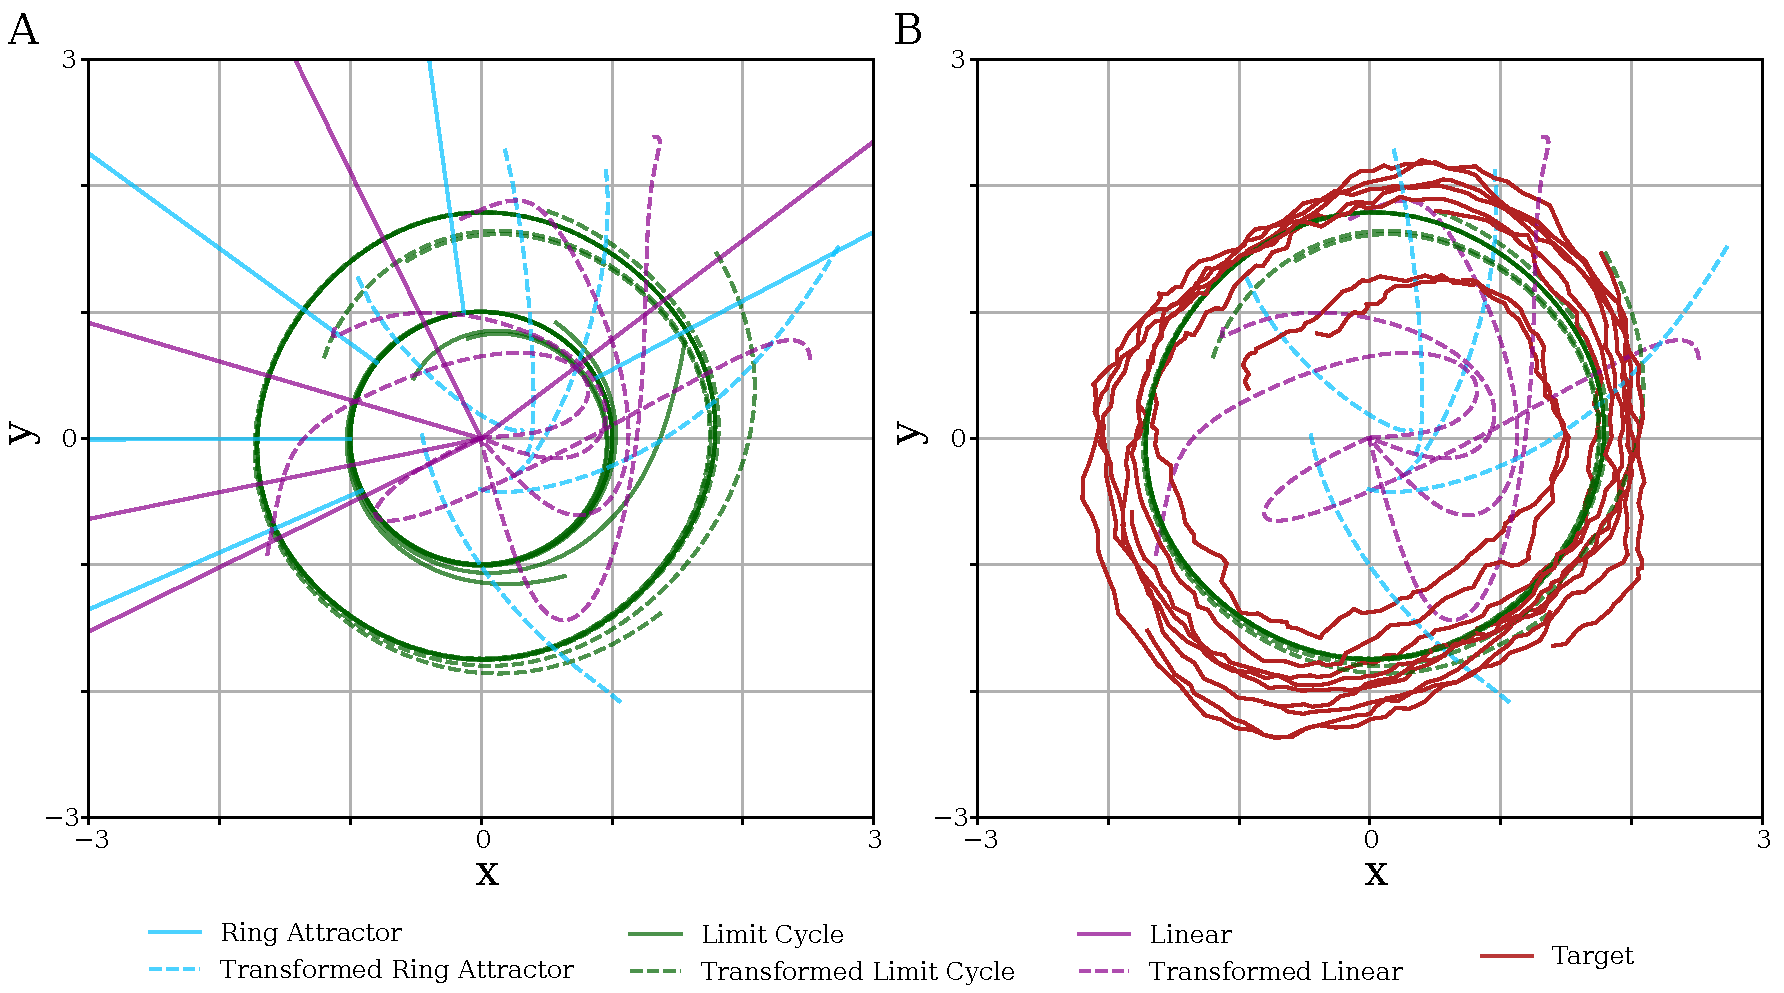
\includegraphics[width=.9\linewidth]{all_motifs_vdp_noisy_var1_ntraj5_ai}
    \caption{Comparison of fitting different motifs to the noisy trajectories generated by a Van der Pol oscillator. The motifs considered in the fitting process include a ring attractor, limit cycle, and fixed point/linear system, sourced from a predefined motif library. The fitting is evaluated based on how well each motif captures the dynamics of the noisy oscillatory data.}
    \label{fig:all_motifs_vdp}
\end{figure}

\subsubsection{Lorenz stable limit cycle}
\citep{lorenz1963deterministic}
If $\rho>313$, then the unique stable limit cycle is an attractor in the Lorenz system\citep{gaiko2014global}.


\subsubsection{Sel'kov}
\citep{selkov1968self}




\subsection{Approximate continuous attractors}
\subsubsection{Line attractor}

\subsubsection{Ring attractor}
\paragraph{Homeomorphism based perturbation}


\paragraph{Vector field based perturbation}
 A smooth perturbation is sampled from a zero-mean Gaussian process with RBF kernel $k(x, x') = \sigma^2 \exp(-\|x - x'\|^2 / 2\ell^2)$, where $\ell$ is drawn uniformly from $[0.1, 1.0]$.
 The perturbation is normalized to have fixed norm.
%LC: a rotational term $(-y, x)$ can be added to the perturbation before normalization to inject limit-cycle-like structure.



\newpage
\section{Architectures}\label{sec:architectures}
\subsection{Neural Ordinary Differential Equations (Neural ODEs)}\label{sec:node}
\citep{chen2018neural,massaroli2020dissecting}
A Neural Ordinary Differential Equation (Neural ODE) is a continuous-time model where the evolution of a system is governed by an ordinary differential equation (ODE) with a neural network defining the dynamics. Specifically, let \( x(t) \in \mathbb{R}^d \) be the state of the system at time \( t \). The evolution of \( x(t) \) is described by the differential equation:
\begin{equation}
    \frac{d}{dt} x(t) = f_\Theta(x(t), t),
\end{equation}
where \( f_\Theta(x(t), t) \) is a neural network parameterized by \( \Theta \), and typically \( f_\Theta \) does not explicitly depend on time \( t \) (i.e., it is a time-invariant system).
 The solution to this equation can is using the Runge-Kutta numerical integration method, with initial condition \( x(0) = x_0 \).

\paragraph{Other proposals}
Neural manifold ordinary differential equations \citep{lou2020neural}.

\subsection{Invertible ResNet}
The basic unit of an Invertible ResNet is the \textit{Invertible ResNet Block}, which operates by splitting the input \( x \in \mathbb{R}^d \) into two parts, \( x_1 \) and \( x_2 \), and applying a transformation only to \( x_1 \). The output is:
\[
 \begin{bmatrix} x_1 + f(x_1) \\ x_2 \end{bmatrix},
\]
where \( f(x_1) = W_2 \cdot \text{ELU}(W_1 \cdot x_1 + b_1) + b_2 \) is a fully connected transformation. %other activation functions?
The block is initialized with identity mapping to ensure invertibility, where \( W_2 = 0 \) and \( W_1 \) is initialized using Kaiming uniform.

The Invertible ResNet consists of stacking multiple Invertible ResNet Blocks. For input \( x \), the forward pass is:
\[
y = \text{InvertibleResNet}(x) = \text{Block}_L(\dots \text{Block}_1(x)),
\]
and the inverse is computed by reversing the block order:
\[
x = \text{InvertibleResNet}^{-1}(y) = \text{Block}_1^{-1}(\dots \text{Block}_L^{-1}(y)).
\]

This structure guarantees that the network is bijective, preserving the volume and making it suitable for density estimation and transformations in generative models.

%\subsection{Normalizing flow}


%\subsection{Naive MLP}
%\begin{tikzpicture}[
%    node distance=0.5cm,
%    neuron/.style={circle, draw, minimum size=0.6cm},
%    layer label/.style={font=\small, anchor=west},
%    every node/.append style={font=\small}
%  ]
%
%  % Input Layer (2 units)
%  \node[layer label] at (-.5, 0.3) {Input};
%  \foreach \i in {1,2} {
%    \node[neuron] (i\i) at (0, -\i) {};
%  }
%
%  % Hidden Layer 1 (8 units, condensed)
%  \node[layer label] at (1.5, 0.3) {$\tanh$};
%  \foreach \i/\y in {1/0.75,3/2.25} {
%    \node[neuron] (h1\i) at (2, -\y) {};
%  }
%  \node at (2, -1.5) {\vdots};
%
%  % Hidden Layer 2 (16 units, condensed)
%  \node[layer label] at (4., 0.3) {$\tanh$};
%  \foreach \i/\y in {1/0.75,3/2.25} {
%    \node[neuron] (h2\i) at (4.5, -\y) {};
%  }
%  \node at (4.5, -1.5) {\vdots};
%
%  % Output Layer (2 units)
%  \node[layer label] at (6.5, 0.3) {Output};
%  \foreach \i in {1,2} {
%    \node[neuron] (o\i) at (6.5, -\i) {};
%  }
%
%  % Connections (sparse for clarity)
%  \foreach \i in {1,2} {
%    \foreach \j in {1,3} {
%      \draw[->] (i\i) -- (h1\j);
%    }
%  }
%
%  \foreach \i in {1,3} {
%    \foreach \j in {1,3} {
%      \draw[->] (h1\i) -- (h2\j);
%    }
%  }
%
%  \foreach \i in {1,3} {
%    \foreach \j in {1,2} {
%      \draw[->] (h2\i) -- (o\j);
%    }
%  }
%
%\end{tikzpicture}



\newpage
\section{Training}

\subsection{Training parameters}



\subsection{Cross-validation}

\subsubsection{Validation data}

\subsubsection{Regularization}

\newpage
\section{Analysis}
\subsection{Comparing and evaluating}

\subsubsection{Jacobian}


\subsubsection{Invariant manifold}
\paragraph{Hausdorff distance}
\[
d_H(A, B) = \max\left\{ \sup_{a \in A} \inf_{b \in B} \|a - b\|, \sup_{b \in B} \inf_{a \in A} \|b - a\| \right\}
\]


\newpage
\section*{NeurIPS Paper Checklist}
%
%%%% BEGIN INSTRUCTIONS %%%
%The checklist is designed to encourage best practices for responsible machine learning research, addressing issues of reproducibility, transparency, research ethics, and societal impact. Do not remove the checklist: {\bf The papers not including the checklist will be desk rejected.} The checklist should follow the references and follow the (optional) supplemental material.  The checklist does NOT count towards the page
%limit. 
%
%Please read the checklist guidelines carefully for information on how to answer these questions. For each question in the checklist:
%\begin{itemize}
%    \item You should answer \answerYes{}, \answerNo{}, or \answerNA{}.
%    \item \answerNA{} means either that the question is Not Applicable for that particular paper or the relevant information is Not Available.
%    \item Please provide a short (1–2 sentence) justification right after your answer (even for NA). 
%   % \item {\bf The papers not including the checklist will be desk rejected.}
%\end{itemize}
%
%{\bf The checklist answers are an integral part of your paper submission.} They are visible to the reviewers, area chairs, senior area chairs, and ethics reviewers. You will be asked to also include it (after eventual revisions) with the final version of your paper, and its final version will be published with the paper.
%
%The reviewers of your paper will be asked to use the checklist as one of the factors in their evaluation. While "\answerYes{}" is generally preferable to "\answerNo{}", it is perfectly acceptable to answer "\answerNo{}" provided a proper justification is given (e.g., "error bars are not reported because it would be too computationally expensive" or "we were unable to find the license for the dataset we used"). In general, answering "\answerNo{}" or "\answerNA{}" is not grounds for rejection. While the questions are phrased in a binary way, we acknowledge that the true answer is often more nuanced, so please just use your best judgment and write a justification to elaborate. All supporting evidence can appear either in the main paper or the supplemental material, provided in appendix. If you answer \answerYes{} to a question, in the justification please point to the section(s) where related material for the question can be found.
%
%IMPORTANT, please:
%\begin{itemize}
%    \item {\bf Delete this instruction block, but keep the section heading ``NeurIPS Paper Checklist"},
%    \item  {\bf Keep the checklist subsection headings, questions/answers and guidelines below.}
%    \item {\bf Do not modify the questions and only use the provided macros for your answers}.
%\end{itemize} 
% 
%
%%%% END INSTRUCTIONS %%%


\begin{enumerate}

\item {\bf Claims}
    \item[] Question: Do the main claims made in the abstract and introduction accurately reflect the paper's contributions and scope?
    \item[] Answer: \answerYes{} % Replace by \answerYes{}, \answerNo{}, or \answerNA{}.
    \item[] Justification: \justificationTODO{}
    \item[] Guidelines:
    \begin{itemize}
        \item The answer NA means that the abstract and introduction do not include the claims made in the paper.
        \item The abstract and/or introduction should clearly state the claims made, including the contributions made in the paper and important assumptions and limitations. A No or NA answer to this question will not be perceived well by the reviewers. 
        \item The claims made should match theoretical and experimental results, and reflect how much the results can be expected to generalize to other settings. 
        \item It is fine to include aspirational goals as motivation as long as it is clear that these goals are not attained by the paper. 
    \end{itemize}

\item {\bf Limitations}
    \item[] Question: Does the paper discuss the limitations of the work performed by the authors?
    \item[] Answer: \answerTODO{} % Replace by \answerYes{}, \answerNo{}, or \answerNA{}.
    \item[] Justification: \justificationTODO{}
    \item[] Guidelines:
    \begin{itemize}
        \item The answer NA means that the paper has no limitation while the answer No means that the paper has limitations, but those are not discussed in the paper. 
        \item The authors are encouraged to create a separate "Limitations" section in their paper.
        \item The paper should point out any strong assumptions and how robust the results are to violations of these assumptions (e.g., independence assumptions, noiseless settings, model well-specification, asymptotic approximations only holding locally). The authors should reflect on how these assumptions might be violated in practice and what the implications would be.
        \item The authors should reflect on the scope of the claims made, e.g., if the approach was only tested on a few datasets or with a few runs. In general, empirical results often depend on implicit assumptions, which should be articulated.
        \item The authors should reflect on the factors that influence the performance of the approach. For example, a facial recognition algorithm may perform poorly when image resolution is low or images are taken in low lighting. Or a speech-to-text system might not be used reliably to provide closed captions for online lectures because it fails to handle technical jargon.
        \item The authors should discuss the computational efficiency of the proposed algorithms and how they scale with dataset size.
        \item If applicable, the authors should discuss possible limitations of their approach to address problems of privacy and fairness.
        \item While the authors might fear that complete honesty about limitations might be used by reviewers as grounds for rejection, a worse outcome might be that reviewers discover limitations that aren't acknowledged in the paper. The authors should use their best judgment and recognize that individual actions in favor of transparency play an important role in developing norms that preserve the integrity of the community. Reviewers will be specifically instructed to not penalize honesty concerning limitations.
    \end{itemize}

\item {\bf Theory assumptions and proofs}
    \item[] Question: For each theoretical result, does the paper provide the full set of assumptions and a complete (and correct) proof?
    \item[] Answer: \answerTODO{} % Replace by \answerYes{}, \answerNo{}, or \answerNA{}.
    \item[] Justification: \justificationTODO{}
    \item[] Guidelines:
    \begin{itemize}
        \item The answer NA means that the paper does not include theoretical results. 
        \item All the theorems, formulas, and proofs in the paper should be numbered and cross-referenced.
        \item All assumptions should be clearly stated or referenced in the statement of any theorems.
        \item The proofs can either appear in the main paper or the supplemental material, but if they appear in the supplemental material, the authors are encouraged to provide a short proof sketch to provide intuition. 
        \item Inversely, any informal proof provided in the core of the paper should be complemented by formal proofs provided in appendix or supplemental material.
        \item Theorems and Lemmas that the proof relies upon should be properly referenced. 
    \end{itemize}

    \item {\bf Experimental result reproducibility}
    \item[] Question: Does the paper fully disclose all the information needed to reproduce the main experimental results of the paper to the extent that it affects the main claims and/or conclusions of the paper (regardless of whether the code and data are provided or not)?
    \item[] Answer: \answerTODO{} % Replace by \answerYes{}, \answerNo{}, or \answerNA{}.
    \item[] Justification: \justificationTODO{}
    \item[] Guidelines:
    \begin{itemize}
        \item The answer NA means that the paper does not include experiments.
        \item If the paper includes experiments, a No answer to this question will not be perceived well by the reviewers: Making the paper reproducible is important, regardless of whether the code and data are provided or not.
        \item If the contribution is a dataset and/or model, the authors should describe the steps taken to make their results reproducible or verifiable. 
        \item Depending on the contribution, reproducibility can be accomplished in various ways. For example, if the contribution is a novel architecture, describing the architecture fully might suffice, or if the contribution is a specific model and empirical evaluation, it may be necessary to either make it possible for others to replicate the model with the same dataset, or provide access to the model. In general. releasing code and data is often one good way to accomplish this, but reproducibility can also be provided via detailed instructions for how to replicate the results, access to a hosted model (e.g., in the case of a large language model), releasing of a model checkpoint, or other means that are appropriate to the research performed.
        \item While NeurIPS does not require releasing code, the conference does require all submissions to provide some reasonable avenue for reproducibility, which may depend on the nature of the contribution. For example
        \begin{enumerate}
            \item If the contribution is primarily a new algorithm, the paper should make it clear how to reproduce that algorithm.
            \item If the contribution is primarily a new model architecture, the paper should describe the architecture clearly and fully.
            \item If the contribution is a new model (e.g., a large language model), then there should either be a way to access this model for reproducing the results or a way to reproduce the model (e.g., with an open-source dataset or instructions for how to construct the dataset).
            \item We recognize that reproducibility may be tricky in some cases, in which case authors are welcome to describe the particular way they provide for reproducibility. In the case of closed-source models, it may be that access to the model is limited in some way (e.g., to registered users), but it should be possible for other researchers to have some path to reproducing or verifying the results.
        \end{enumerate}
    \end{itemize}


\item {\bf Open access to data and code}
    \item[] Question: Does the paper provide open access to the data and code, with sufficient instructions to faithfully reproduce the main experimental results, as described in supplemental material?
    \item[] Answer: \answerTODO{} % Replace by \answerYes{}, \answerNo{}, or \answerNA{}.
    \item[] Justification: \justificationTODO{}
    \item[] Guidelines:
    \begin{itemize}
        \item The answer NA means that paper does not include experiments requiring code.
        \item Please see the NeurIPS code and data submission guidelines (\url{https://nips.cc/public/guides/CodeSubmissionPolicy}) for more details.
        \item While we encourage the release of code and data, we understand that this might not be possible, so “No” is an acceptable answer. Papers cannot be rejected simply for not including code, unless this is central to the contribution (e.g., for a new open-source benchmark).
        \item The instructions should contain the exact command and environment needed to run to reproduce the results. See the NeurIPS code and data submission guidelines (\url{https://nips.cc/public/guides/CodeSubmissionPolicy}) for more details.
        \item The authors should provide instructions on data access and preparation, including how to access the raw data, preprocessed data, intermediate data, and generated data, etc.
        \item The authors should provide scripts to reproduce all experimental results for the new proposed method and baselines. If only a subset of experiments are reproducible, they should state which ones are omitted from the script and why.
        \item At submission time, to preserve anonymity, the authors should release anonymized versions (if applicable).
        \item Providing as much information as possible in supplemental material (appended to the paper) is recommended, but including URLs to data and code is permitted.
    \end{itemize}


\item {\bf Experimental setting/details}
    \item[] Question: Does the paper specify all the training and test details (e.g., data splits, hyperparameters, how they were chosen, type of optimizer, etc.) necessary to understand the results?
    \item[] Answer: \answerTODO{} % Replace by \answerYes{}, \answerNo{}, or \answerNA{}.
    \item[] Justification: \justificationTODO{}
    \item[] Guidelines:
    \begin{itemize}
        \item The answer NA means that the paper does not include experiments.
        \item The experimental setting should be presented in the core of the paper to a level of detail that is necessary to appreciate the results and make sense of them.
        \item The full details can be provided either with the code, in appendix, or as supplemental material.
    \end{itemize}

\item {\bf Experiment statistical significance}
    \item[] Question: Does the paper report error bars suitably and correctly defined or other appropriate information about the statistical significance of the experiments?
    \item[] Answer: \answerTODO{} % Replace by \answerYes{}, \answerNo{}, or \answerNA{}.
    \item[] Justification: \justificationTODO{}
    \item[] Guidelines:
    \begin{itemize}
        \item The answer NA means that the paper does not include experiments.
        \item The authors should answer "Yes" if the results are accompanied by error bars, confidence intervals, or statistical significance tests, at least for the experiments that support the main claims of the paper.
        \item The factors of variability that the error bars are capturing should be clearly stated (for example, train/test split, initialization, random drawing of some parameter, or overall run with given experimental conditions).
        \item The method for calculating the error bars should be explained (closed form formula, call to a library function, bootstrap, etc.)
        \item The assumptions made should be given (e.g., Normally distributed errors).
        \item It should be clear whether the error bar is the standard deviation or the standard error of the mean.
        \item It is OK to report 1-sigma error bars, but one should state it. The authors should preferably report a 2-sigma error bar than state that they have a 96\% CI, if the hypothesis of Normality of errors is not verified.
        \item For asymmetric distributions, the authors should be careful not to show in tables or figures symmetric error bars that would yield results that are out of range (e.g. negative error rates).
        \item If error bars are reported in tables or plots, The authors should explain in the text how they were calculated and reference the corresponding figures or tables in the text.
    \end{itemize}

\item {\bf Experiments compute resources}
    \item[] Question: For each experiment, does the paper provide sufficient information on the computer resources (type of compute workers, memory, time of execution) needed to reproduce the experiments?
    \item[] Answer: \answerTODO{} % Replace by \answerYes{}, \answerNo{}, or \answerNA{}.
    \item[] Justification: \justificationTODO{}
    \item[] Guidelines:
    \begin{itemize}
        \item The answer NA means that the paper does not include experiments.
        \item The paper should indicate the type of compute workers CPU or GPU, internal cluster, or cloud provider, including relevant memory and storage.
        \item The paper should provide the amount of compute required for each of the individual experimental runs as well as estimate the total compute. 
        \item The paper should disclose whether the full research project required more compute than the experiments reported in the paper (e.g., preliminary or failed experiments that didn't make it into the paper). 
    \end{itemize}
    
\item {\bf Code of ethics}
    \item[] Question: Does the research conducted in the paper conform, in every respect, with the NeurIPS Code of Ethics \url{https://neurips.cc/public/EthicsGuidelines}?
    \item[] Answer: \answerTODO{} % Replace by \answerYes{}, \answerNo{}, or \answerNA{}.
    \item[] Justification: \justificationTODO{}
    \item[] Guidelines:
    \begin{itemize}
        \item The answer NA means that the authors have not reviewed the NeurIPS Code of Ethics.
        \item If the authors answer No, they should explain the special circumstances that require a deviation from the Code of Ethics.
        \item The authors should make sure to preserve anonymity (e.g., if there is a special consideration due to laws or regulations in their jurisdiction).
    \end{itemize}


\item {\bf Broader impacts}
    \item[] Question: Does the paper discuss both potential positive societal impacts and negative societal impacts of the work performed?
    \item[] Answer: \answerTODO{} % Replace by \answerYes{}, \answerNo{}, or \answerNA{}.
    \item[] Justification: \justificationTODO{}
    \item[] Guidelines:
    \begin{itemize}
        \item The answer NA means that there is no societal impact of the work performed.
        \item If the authors answer NA or No, they should explain why their work has no societal impact or why the paper does not address societal impact.
        \item Examples of negative societal impacts include potential malicious or unintended uses (e.g., disinformation, generating fake profiles, surveillance), fairness considerations (e.g., deployment of technologies that could make decisions that unfairly impact specific groups), privacy considerations, and security considerations.
        \item The conference expects that many papers will be foundational research and not tied to particular applications, let alone deployments. However, if there is a direct path to any negative applications, the authors should point it out. For example, it is legitimate to point out that an improvement in the quality of generative models could be used to generate deepfakes for disinformation. On the other hand, it is not needed to point out that a generic algorithm for optimizing neural networks could enable people to train models that generate Deepfakes faster.
        \item The authors should consider possible harms that could arise when the technology is being used as intended and functioning correctly, harms that could arise when the technology is being used as intended but gives incorrect results, and harms following from (intentional or unintentional) misuse of the technology.
        \item If there are negative societal impacts, the authors could also discuss possible mitigation strategies (e.g., gated release of models, providing defenses in addition to attacks, mechanisms for monitoring misuse, mechanisms to monitor how a system learns from feedback over time, improving the efficiency and accessibility of ML).
    \end{itemize}
    
\item {\bf Safeguards}
    \item[] Question: Does the paper describe safeguards that have been put in place for responsible release of data or models that have a high risk for misuse (e.g., pretrained language models, image generators, or scraped datasets)?
    \item[] Answer: \answerTODO{} % Replace by \answerYes{}, \answerNo{}, or \answerNA{}.
    \item[] Justification: \justificationTODO{}
    \item[] Guidelines:
    \begin{itemize}
        \item The answer NA means that the paper poses no such risks.
        \item Released models that have a high risk for misuse or dual-use should be released with necessary safeguards to allow for controlled use of the model, for example by requiring that users adhere to usage guidelines or restrictions to access the model or implementing safety filters. 
        \item Datasets that have been scraped from the Internet could pose safety risks. The authors should describe how they avoided releasing unsafe images.
        \item We recognize that providing effective safeguards is challenging, and many papers do not require this, but we encourage authors to take this into account and make a best faith effort.
    \end{itemize}

\item {\bf Licenses for existing assets}
    \item[] Question: Are the creators or original owners of assets (e.g., code, data, models), used in the paper, properly credited and are the license and terms of use explicitly mentioned and properly respected?
    \item[] Answer: \answerTODO{} % Replace by \answerYes{}, \answerNo{}, or \answerNA{}.
    \item[] Justification: \justificationTODO{}
    \item[] Guidelines:
    \begin{itemize}
        \item The answer NA means that the paper does not use existing assets.
        \item The authors should cite the original paper that produced the code package or dataset.
        \item The authors should state which version of the asset is used and, if possible, include a URL.
        \item The name of the license (e.g., CC-BY 4.0) should be included for each asset.
        \item For scraped data from a particular source (e.g., website), the copyright and terms of service of that source should be provided.
        \item If assets are released, the license, copyright information, and terms of use in the package should be provided. For popular datasets, \url{paperswithcode.com/datasets} has curated licenses for some datasets. Their licensing guide can help determine the license of a dataset.
        \item For existing datasets that are re-packaged, both the original license and the license of the derived asset (if it has changed) should be provided.
        \item If this information is not available online, the authors are encouraged to reach out to the asset's creators.
    \end{itemize}

\item {\bf New assets}
    \item[] Question: Are new assets introduced in the paper well documented and is the documentation provided alongside the assets?
    \item[] Answer: \answerTODO{} % Replace by \answerYes{}, \answerNo{}, or \answerNA{}.
    \item[] Justification: \justificationTODO{}
    \item[] Guidelines:
    \begin{itemize}
        \item The answer NA means that the paper does not release new assets.
        \item Researchers should communicate the details of the dataset/code/model as part of their submissions via structured templates. This includes details about training, license, limitations, etc. 
        \item The paper should discuss whether and how consent was obtained from people whose asset is used.
        \item At submission time, remember to anonymize your assets (if applicable). You can either create an anonymized URL or include an anonymized zip file.
    \end{itemize}

\item {\bf Crowdsourcing and research with human subjects}
    \item[] Question: For crowdsourcing experiments and research with human subjects, does the paper include the full text of instructions given to participants and screenshots, if applicable, as well as details about compensation (if any)? 
    \item[] Answer: \answerTODO{} % Replace by \answerYes{}, \answerNo{}, or \answerNA{}.
    \item[] Justification: \justificationTODO{}
    \item[] Guidelines:
    \begin{itemize}
        \item The answer NA means that the paper does not involve crowdsourcing nor research with human subjects.
        \item Including this information in the supplemental material is fine, but if the main contribution of the paper involves human subjects, then as much detail as possible should be included in the main paper. 
        \item According to the NeurIPS Code of Ethics, workers involved in data collection, curation, or other labor should be paid at least the minimum wage in the country of the data collector. 
    \end{itemize}

\item {\bf Institutional review board (IRB) approvals or equivalent for research with human subjects}
    \item[] Question: Does the paper describe potential risks incurred by study participants, whether such risks were disclosed to the subjects, and whether Institutional Review Board (IRB) approvals (or an equivalent approval/review based on the requirements of your country or institution) were obtained?
    \item[] Answer: \answerTODO{} % Replace by \answerYes{}, \answerNo{}, or \answerNA{}.
    \item[] Justification: \justificationTODO{}
    \item[] Guidelines:
    \begin{itemize}
        \item The answer NA means that the paper does not involve crowdsourcing nor research with human subjects.
        \item Depending on the country in which research is conducted, IRB approval (or equivalent) may be required for any human subjects research. If you obtained IRB approval, you should clearly state this in the paper. 
        \item We recognize that the procedures for this may vary significantly between institutions and locations, and we expect authors to adhere to the NeurIPS Code of Ethics and the guidelines for their institution. 
        \item For initial submissions, do not include any information that would break anonymity (if applicable), such as the institution conducting the review.
    \end{itemize}

\item {\bf Declaration of LLM usage}
    \item[] Question: Does the paper describe the usage of LLMs if it is an important, original, or non-standard component of the core methods in this research? Note that if the LLM is used only for writing, editing, or formatting purposes and does not impact the core methodology, scientific rigorousness, or originality of the research, declaration is not required.
    %this research? 
    \item[] Answer: \answerTODO{} % Replace by \answerYes{}, \answerNo{}, or \answerNA{}.
    \item[] Justification: \justificationTODO{}
    \item[] Guidelines:
    \begin{itemize}
        \item The answer NA means that the core method development in this research does not involve LLMs as any important, original, or non-standard components.
        \item Please refer to our LLM policy (\url{https://neurips.cc/Conferences/2025/LLM}) for what should or should not be described.
    \end{itemize}

\end{enumerate}


\end{document}

